\chapter{Fundamentos te\'orico-conceptuales}\label{chapter:bi-industry-4.0}

\section{Evolución de las bases de datos}

La información es un recurso estratégico producido en grandes volúmenes durante la era moderna, donde las bases de datos se han consolidado como una herramienta esencial para almacenar y recuperar información de manera eficiente.

Aunque el término \textit{base de datos} fue formalmente introducido en el ámbito matemático y computacional durante la década de 1960, 
la práctica de guardar y organizar datos ha sido una piedra angular en el desarrollo de la civilización humana, la ciencia y la tecnología. En épocas tempranas, este concepto se manifestaba a través de bibliotecas y archivos, que almacenaban grandes volúmenes de información en libros y documentos físicos. Estos sistemas tradicionales guardan una notable analogía con las bases de datos actuales, diferenciándose principalmente en que los datos ahora se gestionan en formato digital, lo que permite un acceso y manejo más ágil y versátil.

La primera revolución de las bases de datos comenzó en la década de 1960, cuando el uso de computadoras se convirtió en una opción rentable para las organizaciones privadas.
% El surgimiento de las computadoras electrónicas marcó la primera re- volución de las bases de datos. 
El desarrollo de aplicaciones para la administración de datos 
empezó a requerir establecer control sobre un conjunto propio de datos y 
la implementación de código más sofisticado para satisfacer nuevos y más complejos requerimientos. 
Así surge la idea de separar la lógica de gestión de los datos de la lógica de la aplicación, 
que derivó en el desarrollo de los primeros Sistemas de Gestión de Bases de Datos (SGBD). Las bases
de datos más populares de esta década, una basada en el modelo jerárquico llamada IMS \cite{hubbard1986ims} y una basada
en un modelo de redes llamada CODASYL \cite{taylor1976codasyl}, forzaban a la definición de una estructura en los datos muy poco flexible y, 
aunque dominaron el mercado de bases de datos hasta finales de los años 70’s, no tardaron en emerger sus desventajas e inconvenientes como la inflexibilidad e inexpresividad en la consultas \cite{harrison2015next}. 
Además, eran muy difíciles de utilizar pues al carecer de una base teórica la forma de lograr la consistencia lógica era por medio de la programación.

En 1970, Edgar F. Codd, un matemático y programador que trabajaba en las oficinas de IBM, publicó un
artículo bajo el título \textit{``A Relational Model of Data for Large Shared Data Banks''} \cite{codd1970relational} en el que describe un tipo de bases de datos basadas
en el nuevo modelo relacional, esta teoría marcó el inicio de la segunda revolución en las bases de datos cambiando
radicalmente la tecnología para su administración.
Las bases de datos relacionales están construidas sobre un modelo matemático formal, 
que representa los datos y las interrelaciones entre ellos mediante la relación, 
una estructura de datos que puede visualizarse como una tabla en términos de implementación. 
Codd introdujo el concepto de consistencia, para referirse al estado que alcanza una base de datos cuando satisface un conjunto de restricciones, denominadas en el contexto relacional, 
como restricciones de integridad. Las restricciones de integridad proporcionan las bases lógicas para asegurar la correctitud y veracidad de los datos durante la manipulación de los mismos.

Durante la década de 1980 el \textit{American National Standards Institute} y la \textit{International Organization for Standardization} reconocieron SQL (\textit{Structured Query Language})
como lenguaje de consulta estandar \cite{chamberlin2012early}. 
La bases de datos relacionales se convirtieron en un éxito comercial a medida que las computadoras se abarataban y sus ventas se
incrementaban, agrandando el potencial mercado de bases de datos. Por otro lado, esto causó un gran declive en la popularidad
de los modelos jerárquicos y de redes.

Al comienzo de los años 2000s las bases se datos relacionales parecían inamovibles en el mercado. 
Fueron adoptadas y constituyeron durante años sino la única, la más popular alternativa para el almacenamiento de grandes volúmenes de datos. 
Aunque hubo significativos y contribuyentes avances dentro del modelo relacional, no había signos de la ocurrencia de un gran cambio en este campo \cite{harrison2015next}.

La llegada y asentamiento de la Web, la compra de computadoras personales y la creciente inversión en
el comercio electrónico llevó a un crecimiento exponencial de la industria de bases de datos, marcando
la era de las aplicaciones masivas web-scale \cite{harrison2015next}. A pesar de su popularidad y eficacia,
las limitaciones del modelo relacional empazaron a tornarse un problema cada vez mayor, a medida que grandes
compañías como Google, Facebook, Yahoo! y Amazon comenzaron a tratar con enormes volúmenes de datos y de
usuarios. 


El crecimiento de estas aplicaciones generó nuevos retos, como el manejo de un gran volumen de operaciones de lectura y escritura, baja latencia en los tiempos de respuesta y alta disponibilidad; requisitos muy difíciles de lograr con el solo uso de bases de datos relacionales.
Lograr algunos de estos objetivos con bases de datos relacionales era posible en ciertos casos, pero con muchas dificultades y costos potencialmente altos \cite{strauch2011nosql}.
Los sistemas relacionales han sido diseñados para residir en un único servidor, formar parte de arquitecturas cliente/servidor y, por ende, para escalar verticalmente (destinando mayores recursos computacionales al único servidor utilizado). 
Esto no niega que sea posible trabajar con bases de datos relacionales distribuidas, 
solo que ello conlleva un esfuerzo adicional, resulta una tarea ardua, engorrosa y, a veces,
imposible para alcanzar los niveles de escalabilidad que requieren las aplicaciones mientras continúan respondiendo sin interrupción a las demandas de los usuarios.
Los SGBD relacionales se caracterizan por el procesamiento transaccional de los datos, basados en los principios ACID \cites*{strauch2011nosql,pokorny2011nosql} que dificultan el escalamiento horizontal (agregar nodos al sistema):.

\begin{itemize}
    \item \textbf{Atomicity (A)}: Unasecuenciadeoperaciones(transacción)seejecutarádel todo o nada.
    \item \textbf{Consistency (C)}: Una transacción no deja la base de datos en un estado inconsistente, no se viola ninguna restricción de integridad.
    \item \textbf{Isolation (I)}: Las transacciones concurrentes son independientes, una no interfiere con otra.
    \item \textbf{Durability (D)}: Los cambios realizados por una transacción serán reverti- dos ante fallas del sistema.
\end{itemize}


Para justificar la incompatibilidad entre los nuevos requerimientos de las aplicaciones web y los principios sobre los que había sido construido el
modelo relacional que utilizaban en su implementación, en el año 2000, el profesor Eric Brewer, de la Universidad de California, Berkeley, planteó que es imposible 
para un sistema de base de datos distribuido satisfacer simultáneamente la consistencia, la disponibilidad y la tolerancia a particiones. 
Esta conjetura se conviertió en un teorema dos años después cuando se publica una demostración formal y pasa a conocerse en la literatura como el Teorema CAP \cite{gilbert2012perspectives}, por sus siglas en inglés \textit{Consistency}, \textit{Availability} y \textit{Partition Tolerance} (véase figura \ref{fig:cap-theorem}).

\begin{figure}[h!]
    \centering
    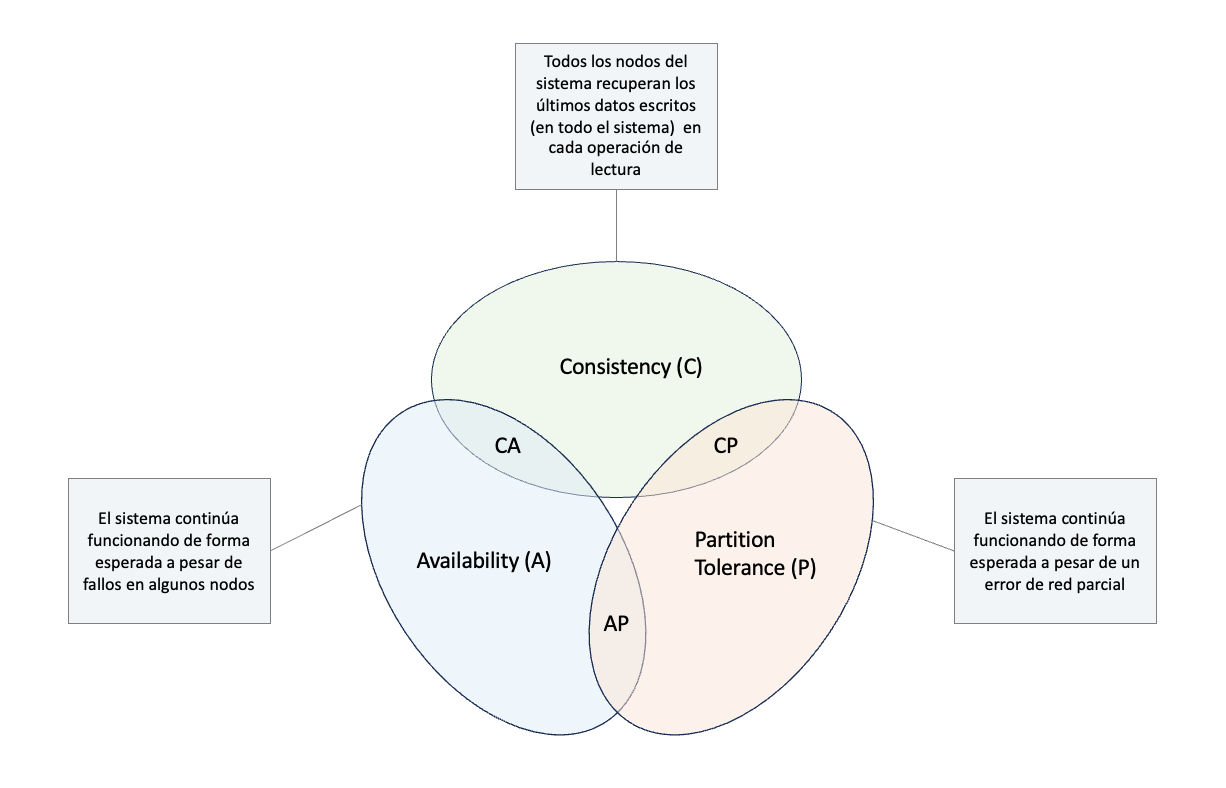
\includegraphics[width=0.7\textwidth]{Images/cap-theorem.png}
    \caption{Diagrama de Venn del Teorema CAP}
    \label{fig:cap-theorem}
\end{figure}


Las soluciones para lograr el escalamiento horizontal en las aplicaciones se basan en la partición de los datos, lo que lleva a deducir que la presencia de la tolerancia a particiones en los sistemas de bases de datos es un requerimiento, más que una opción. 
El abandono de la consistencia mejora en gran medida la disponibilidad del sistema, mientras que su elección por encima de la disponibilidad implica, bajo ciertas circunstancias, que el sistema no estará disponible \cite{vogels2008eventually}. 
Dependiendo de las necesidades particulares de una aplicación, algunas de estas características son más importantes que otras \cite{pokorny2011nosql}.
Esta dicotomía introduce el concepto de consistencia eventual, esto significa que el sistema aboga por la disponibilidad, por lo que las demandas de los clientes serán atendidas instantáneamente, pero los cambios no se reflejarán de igual forma a través de todo el sistema sino que se efectuarán ocasionalmente \cite{vogels2008eventually}.
Esta variante, evidentemente no cumple con las propiedades ACID de los sistemas relacionales, sino que se incorpora a otro conjunto de principios conocidos como BASE \cites*{pokorny2011nosql,vogels2008eventually}:

\begin{itemize}
    \item \textbf{Basically Available (BA)}: Pueden existir fallas parciales en algunos nodos del sistema distribuido, pero aun así el resto del sistema continúa su función.
    \item \textbf{Soft state (S)}: Esta expresión quiere decir que los datos serán reemplazados por datos más recientes. La base de datos no es consistente todo el tiempo. Esta propiedad se superpone a la tercera.
    \item \textbf{Eventual consistency (E)}: La base de datos alcanzará consistencia eventualmente, puede haber instantes de tiempo que no sea consistente.
\end{itemize}


Con el fin de superar las limitaciones del modelo relacional surgieron las bases de datos NoSQL, que tienen como fundamento los principios BASE.
El término ``NoSQL'' quiere decir \textit{``Not only SQL''} y se refiere a una clase de SGBDs identificados por su no adherencia al modelo relacional,
intentando resolver los problemas de escalabilidad y disponibilidad contra los problemas de atomicidad y consistencia.
Las bases de datos NoSQL usualmente no se construyen sobre tablas y como resultado, generalmente no utilizan SQL para la manipulación de los datos \cite{vaish2013getting}. 
NoSQL no representa una ruptura con el modelo relacional, sino que amplía y modifica sus principios fundamentales, aunque tampoco constituye la mejor solución para todo tipo de problemas \cite{harrison2015next}.
La llegada de este nuevo concepto marca el inicio de la tercera revolución de las bases de datos, en la que no se defiende el uso de solo una arquitectura,
ya que una misma arquitectura de base de datos no puede resolver todos los retos a los que se enfrenta el mundo digital moderno \textit{(One Size Doesn’t Fit All)} \cite{harrison2015next}.
 Esta etapa se caracteriza por aplicaciones desarrolladas en la nube, tecnología móvil, redes sociales e internet de las cosas.
 Asimismo, se constata gran variabilidad en los datos que requiere flexibilidad en los modelos para tratar con datos semi-estructurados y no-estructurados y la 
 necesidad de manejar grandes volúmenes de datos, es por ello que se considera que vivimos en la era de Big Data, un concepto que se ha convertido en una de las tendencias tecnológicas más importantes en la actualidad \cite{sagiroglu2013big}.


\section{Grafos de conocimientos}

\subsection{Teor\'ia de grafos}\label{section:graph-theory}

La teor\'ia de grafos se centra en el estudio de un modelo
matem\'atico propuesto por el matem\'atico Leonhard Euler en el
a\~no 1736 denominado grafo \cite{bondy2008graph}.

\begin{definition}
    Un \textbf{grafo} es un par formado por dos conjuntos $G = (V,E)$, 
    donde \\ $v \in V$ representa un v\'ertice (o nodo) del grafo y $E$ es un conjunto
    de pares no ordenados de elementos de $V$ a los cuales se les llama aristas. $G$ est\'a asociado con una funci\'on de tipado de v\'ertices $f_v: V \to \mathcal{T}^v$ y 
    una funci\'on de tipado de aristas $f_e : E \to \mathcal{T}^e$.  
\end{definition}

\begin{definition}
    Un grafo $G$ es \textbf{dirigido} si la existencia de la arista $\{v_i, v_j\} \in E$ no
    necesariamente implica la existencia de la arista sim\'etrica $\{v_j, v_i\} \in E$.
\end{definition}

\begin{definition}
    Un \textbf{grafo heterog\'eneo} $G_{hete}$ es un grafo tal 
    que $|\mathcal{T}^v| > 1 \vee |\mathcal{T}^e| > 1$. Existen v\'ertices y/o aristas
    de distinto tipo.
\end{definition}

\begin{definition}
    Un \textbf{grafo atributado} $G = (V,E,A,I)$ es una tupla de cuatro
    elementos, donde $V$ es un conjunto
    de v\'ertices, $E$ es un conjunto de aristas, $A$ es un
    conjunto de atributos e $I : V \cup E \to 2^A$ es una
    funci\'on que asigna conjuntos de atributos a los v\'ertices
    y aristas del grafo.
\end{definition}

\begin{definition}
    Un \textbf{grafo de conocimientos} $G_{know} = (V,E)$ es un grafo cuyos v\'ertices
    se consideran \textbf{entidades} y sus aristas son triplas de la forma $<h,r,t>$,
    donde $h, t \in V$ y $r$ representa el tipo de \textbf{relaci\'on} que se establece entre
    ambas entidades. 
\end{definition}



Los grafos pueden ser representados computacionalmente de distintas formas, las formas
m\'as utilizadas son la matriz de adyacencia y las listas de adyacencia.


\begin{definition}
    Dado un grafo $G = (V,E)$ la matriz de adyacencia de $G$ es una matriz
    $M^{|V|\times|V|}$ tal que:
    
    $$
            M_{ij} =
        \left\{
            \begin{array}{ll}
                1  & \mbox{if } \{v_i, v_j\} \in E \\
                0 & \mbox{if } e.o.c
            \end{array}
        \right.
    $$

\end{definition}


\begin{definition}
    Sea un grafo $G = (V,E)$ la lista de adyacencia de un v\'ertice $v \in V$ es el conjunto
    $\{ u \in V : \{v,u\} \in E \}$.
\end{definition}


\subsection{Sistemas de almacenamiento de grafos}

En la actualidad existen dos tipos principales de sistemas de almacenamiento para grafos:
las bases de datos orientadas a grafos y los almacenes RDF \cite{angles2008survey}. 
La principal diferencia de estos
sistemas es la expresividad permitida por su modelo de datos, es decir que tantas características
de un grafo son capaces de implementar (tipado, vértices atributados, aristas atributadas, etc.)

Un almacén RDF es una base de datos diseñada para almacenar, gestionar y consultar datos estructurados en formato RDF (\textit{Resource Description Framework}). 
El modelo RDF representa la información como triplas compuestas por un sujeto, un predicado y un objeto, y fue diseñado para representar los metadatos acerca de los recursos en la \textit{World Wide Web} \cite{manola2004rdf}.
Este formato es fundamental para la web semántica, ya que permite vincular datos de diferentes fuentes y facilitar su interpretación tanto por humanos como por máquinas. Los almacenes RDF se utilizan ampliamente en aplicaciones que requieren interoperabilidad de datos, como gestión de ontologías, motores de búsqueda semánticos, y análisis de grandes volúmenes de datos \cites*{haase2004comparison,decker2005triple,malik2016big}. 
Su propósito principal es permitir un acceso estandarizado a datos semánticos a través de lenguajes como SPARQL \cite{perez2006semantics}.

Una base de datos orientada a grafos es un sistema diseñado para almacenar, gestionar y consultar datos estructurados como grafos, donde las entidades se representan como nodos, las interrelaciones como aristas, y las propiedades asociadas se almacenan como atributos en ambos \cite{angles2008survey}. 
Este modelo es más general que el formato RDF permitiendo representar y analizar estructuras más complejas. 
Las bases de datos de grafos están optimizadas para consultas que implican recorridos o análisis de vecindad, como encontrar rutas más cortas, detectar comunidades o analizar patrones de conectividad \cite{neo4jgraph}. 
Estas bases de datos no implementan un estándar y utilizan lenguajes de consulta propietarios especializados como Cypher, Gremlin o GQL \cite{neo4jcypher}. 
Su propósito principal es ofrecer un enfoque eficiente y flexible para modelar datos interconectados, lo que las hace esenciales en sectores como logística, ciberseguridad, marketing, y análisis de redes complejas \cite{neo4jgraphuses}.

Una comparación más detallada de ambas bases de datos puede ser vista en la tabla \ref{tab:graph-db-comparison-table}.

    \begin{longtable}{|p{3cm}|p{5cm}|p{5cm}|}
        \hline
        \textbf{Aspecto} & \textbf{Bases de datos orientadas a grafos} & \textbf{Almacenes RDF} \\
        \hline
        \endfirsthead
        \caption{Comparación entre bases de datos orientadas a grafos y almacenes RDF}\label{tab:graph-db-comparison-table}\\
        

        \hline
        \textbf{Aspecto} & \textbf{Bases de datos orientadas a grafos} & \textbf{Almacenes RDF} \\
        \hline
        \endhead

        
        \hline
        \multicolumn{3}{|r|}{\textit{Continúa en la siguiente página}} \\
        \hline
        \endfoot
        
        \hline
        \endlastfoot

        
        Modelo de datos & Nodos (entidades), aristas (relaciones) y propiedades. & Tripletas: sujeto, predicado y objeto. Basado en el modelo RDF. \\
        \hline
        Lenguaje de consulta & Cypher, Gremlin, GQL. & SPARQL (estándar de W3C). \\
        \hline
        Flexibilidad del esquema & Esquema flexible, adaptado a datos dinámicos. & Esquema estructurado basado en RDF. \\
        \hline
        Optimización & Diseñadas para consultas rápidas en grafos y análisis de relaciones. & Optimizadas para razonamiento semántico y consultas basadas en tripletas. \\
        \hline
        Propósito principal & Modelado de relaciones complejas y análisis de grafos. & Interoperabilidad y razonamiento sobre datos semánticos. \\
        \hline
        Estándares & No dependen de un estándar universal, varía según el proveedor. & Cumplen con los estándares de W3C (RDF, OWL, SPARQL). \\
        \hline
        Casos de uso & Redes sociales, motores de recomendación, análisis de redes. & Web semántica, gestión de ontologías, datos enlazados. \\
        \hline
        Ejemplos & Neo4j, TigerGraph, ArangoDB. & Apache Jena, Stardog, AllegroGraph. \\
        \hline
    
        \end{longtable}



\section{Productos naturales y química computacional}

Los productos naturales son sustancias producidas por organismos en condiciones naturales, las cuales no han sido modificadas de forma significativa por los humanos. 
La composición de los productos naturales puede incluir un amplio rango de compuestos, constituyendo una reserva de diversidad química prometedora a explorar en búsqueda de sustancias con aplicaciones industriales. 
Actualmente son muy utilizados en diferentes industrias como la farmacéutica, cosmética y agrícola debido a la creciente demanda de opciones más saludables y sostenibles. 
Esto ha motivado al incremento de la investigación con respecto a la química de productos naturales.

En la actualidad la investigación en química se ha convertido cada vez más en un área multidisciplinaria. 
Los avances en bases de datos químicas, inteligencia artificial, visualización y análisis de datos han acelerado el desarrollo de la química computacional, 
la computación tiene un rol creciente dentro de la investigación química. 
Por tanto, se vuelve necesario el conocer las formas de representar y buscar computacionalmente un producto natural, 
así como las herramientas computacionales utilizadas para esto.

\subsection{Representación computacional de productos naturales}

Las estructuras químicas son usualmente representadas como grafos moleculares, 
como fue mencionado en la sección \ref{section:graph-theory} un grafo es una estructura compuesta por un conjunto de vértices conectados por aristas. 
En un grafo molecular los átomos y enlaces son representados por los vértices y las aristas respectivamente, 
además pueden incluir información adicional como el número atómico asociado a cada vértice y el orden del enlace en cada arista. 
El almacenar estas propiedades le permite al grafo representar la estructura de la molécula, es decir, la forma en que los átomos (vértices) están conectados \cite{leach2007introduction}.  

\begin{figure}[h!]
    \centering
    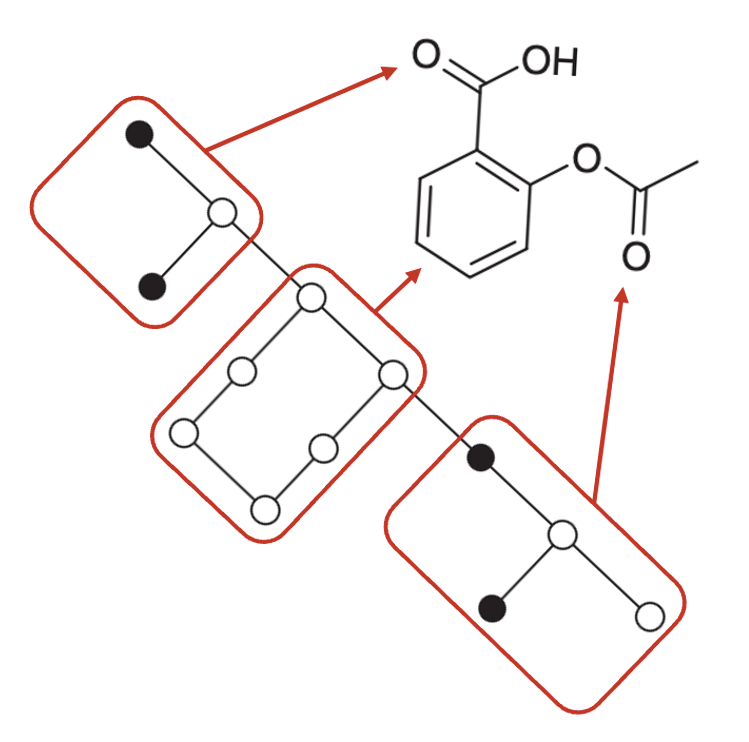
\includegraphics[width=0.5\textwidth]{Images/np-graph-representation.png}
    \caption{Representación de un grafo molecular de la estructura química de la aspirina (acído acetil salicílico)}
    \label{fig:np-graph-representation}
\end{figure}


Una vez representada la molécula como un grafo molecular se debe codificar este grafo en un formato entendible por la computadora. 
Los dos métodos más utilizados en química computacional para dicho propósito son la tabla de conexión y la notación linear. 
Los formatos basados en tablas de conexión usualmente codifican el grafo en dos secciones: la primera sección contiene las propiedades de los átomos y la segunda sección es una tabla de adyacencia entre los vértices la cual representa los enlaces moleculares. 
Estos formatos permiten almacenar una mayor cantidad de información, incluyendo propiedades atómicas, de enlaces y coordenadas de posición para la visualización 2D y 3D de la molécula. 
Por otro lado, los formatos basados en notación lineal utilizan caracteres alfanuméricos para codificar la estructura, siendo una representación más compacta de la tabla de conexión, permitiendo el almacenamiento y transmisión de un mayor número de moléculas \cites*{leach2007introduction,heller2015inchi}. A continuación, se presentan algunos de los formatos más utilizados para la representación computacional de productos naturales.

\begin{itemize}
  \item \textbf{MDL Molfile}: es un formato desarrollado por Molecular Design Limited (MDL) \cite{dalby1992description} el cual utiliza una tabla de conexión para representar la estructura de la molécula. Este formato, particularmente sus versiones V2000 y V3000, es ampliamente utilizado en bases de datos químicas y softwares de visualización molecular debido a su forma estructurada y sencilla de codificar estructuras moleculares en 2D y 3D.
  \item \textbf{International Chemical Identifier} (InChI) \cite{heller2015inchi} es un identificador para sustancias químicas en notación lineal desarrollado bajo el auspicio de la International Union of Pure and Applied Chemistry (IUPAC) y el National Institute of Standards and Technology (NIST) bajo una licencia de código abierto. Este expresa las estructuras químicas en términos de conectividad, equilibrio tautomérico, isótopos, estereoquímica y carga electrónica para producir una cadena única para cada molécula. En la actualidad este identificador es ampliamente utilizado para la integración de distintas piezas de información química, especialmente en servicios orientados a la web.
  \item \textbf{InChI Key} \cite{heller2015inchi} es una versión de 25 caracteres del InChI de una determinada molécula, diseñado para facilitar la búsqueda de compuestos químicos a través de la web. Este identificador es obtenido a través del hashing de una cadena InChI original, lo cual, hoy en día en ciertos casos, puede provocar colisiones de un mismo InChI Key a distintos InChIs. Además, siendo el hash una función de un solo sentido es imposible reconstruir el InChI original y por tanto recuperar la estructura de la molécula a partir del InChI Key.
  \item \textbf{Canonical Simplified Molecular Input Line Entry Specification} (Canonical SMILES) \cite{weininger1988smiles}  es un identificador para sustancias químicas en notación lineal en el cual los átomos y enlaces son representados por símbolos siguiendo reglas establecidas. Para construir un SMILES es necesario recorrer el grafo molecular de forma que cada átomo sea visitado una y solo una vez. Debido a que puede haber múltiples recorridos posibles es necesario generar una representación canónica de la molécula, esto es un orden único de los átomos para un determinado grafo molecular.
  \item Las \textbf{huellas moleculares} son representaciones numéricas de estructuras moleculares codificadas como vectores binarios de longitud fija. Cada bit de una huella molecular representa la presencia de un átomo o sub-estructura específica dentro del compuesto \cite{cereto2015molecular}. 
    \begin{itemize}
        \item \textbf{MACCS Keys} es una huella de 166 bits asociados a la presencia de 166 estructuras definidas en una lista de subestructuras y patrones.
        \item \textbf{Morgan Fingerprint} o \textbf{Extended Connectivity Fingerprint} (ECFP) es un vector binario el cual es obtenido utilizando una función de hash sobre las características topológicas de los átomos y sus enlaces en un radio determinado \cite{rogers2010extended}.
    \end{itemize}
\end{itemize}



\subsection{Métodos computacionales de búsqueda de productos naturales}


Las bases de datos utilizadas para almacenar y buscar la información de las estructuras químicas han tendido hacia la especialización, debido a la naturaleza de los métodos utilizados para representar y manipular las estructuras químicas de forma computacional. Dicha especialización ha llevado a dividir la funcionalidad de búsqueda de moléculas en tres categorías de acuerdo con los objetivos y restricciones de la búsqueda.

\begin{itemize}
    \item La \textbf{búsqueda exacta de estructura} es la tarea más sencilla requiriendo recuperar la información correspondiente con una estructura determinada. La utilización de identificadores de estructuras moleculares como el InChI, SMILES o hashes de estos permite la utilización de estructuras de datos como los índices para obtener de forma eficiente la localización en memoria de la información asociada a la molécula \cite{leach2007introduction}. 
    \item La \textbf{búsqueda de subestructura} es quizás la forma más utilizada para identificar compuestos de interés. Esta búsqueda recupera todas las moléculas en la base de datos que contienen una subestructura determinada. Este problema es equivalente a determinar si un grafo está contenido dentro de otro (isomorfismo de subgrafo), por tanto, métodos de teoría de grafos pueden ser utilizados para realizar esta búsqueda. Existen algoritmos eficientes bien establecidos para buscar isomorfismos de subgrafos, sin embargo, para grandes bases de datos de compuestos químicos es demasiado costoso el utilizar solamente estos algoritmos. Por dicho motivo, la mayoría de las bases de datos realizan la búsqueda en dos etapas: durante la primera se utilizan heurísticas para rápidamente descartar moléculas sin posibilidad de satisfacer la consulta del usuario, las estructuras restantes son analizadas con los algoritmos de grafo durante la segunda fase para obtener el resultado de la consulta \cite{willett2005searching}. 
    \item La \textbf{búsqueda de similaridad} se basa en la utilización de métricas de similitud para comparar moléculas. En general estas métricas intentan estimar la similitud estructural entre un par de moléculas, debido a esto las moléculas son representadas utilizando huellas moleculares que indican las subestructuras presentes dentro de estas. La medida de similitud más utilizada para comparar estructuras representadas por huellas moleculares es el Coeficiente de Tanimoto \cite{bajusz2015tanimoto}. Estas medidas son utilizadas para buscar compuestos con similares actividades biológicas bajo la premisa de “estructuras similares tienen similar actividad biológica”, sin embargo, esta premisa no siempre es verdadera.
\end{itemize}



\subsection{Herramientas de química computacional para el desarrollo de software}

Debido a la existencia de múltiples representaciones para productos naturales se necesita de herramientas capaces de poder convertir estos formatos entre sí, además de poder realizar el cálculo de propiedades a partir de la estructura e incorporar los algoritmos utilizados para la búsqueda de compuestos. Esto ha llevado al surgimiento de distintos paquetes de software especializados para lo química computacional, sin los cuales el trabajo con estructuras se vuelve altamente complicado. A continuación, se presenta una lista de los paquetes más relevantes.

\begin{longtable}{|p{4cm}|p{3cm}|p{3cm}|p{3cm}|}
    \hline
    \textbf{Característica} & \textbf{Open Babel} & \textbf{RDKit} & \textbf{Indigo} \\
    \hline
    \endfirsthead
    
    \hline
    \textbf{Característica} & \textbf{Open Babel} & \textbf{RDKit} & \textbf{Indigo} \\
    \hline
    \endhead
    
    \hline
    \multicolumn{4}{|r|}{\textit{Continúa en la siguiente página}} \\
    \endfoot
    
    \hline
    \endlastfoot
    
    Licencia & GPL-2 Licence & BSD-3 Licence & Apache License version 2.0 \\
    \hline
    Conversión de estructuras & Sí & Sí & Sí \\
    \hline
    Cálculo de huellas moleculares & Sí & Sí & Sí \\
    \hline
    Cálculo de medidas de similaridad & Sí & Sí & Sí \\
    \hline
    Búsqueda de subestructuras & Sí & Sí & Sí \\
    \hline
    Visualización de estructuras & Sí & Sí & Sí \\
    \hline
    Lenguajes soportados & C++ & Python, Java, C\# y JavaScript & .NET, Java, Python, R y WebAssembly \\
    \hline
    Bases de datos soportadas & - & PostgreSQL & Oracle, Microsoft SQL Server y PostgreSQL \\
    \hline
    
    \end{longtable}

\subsection{Bases de datos de productos naturales}
 

    En las últimas décadas, se ha observado un creciente impulso en el desarrollo de una gran variedad de bases de datos relacionadas con productos naturales, con el propósito
    de facilitar el desarrollo de fármacos. Un meticuloso estudio realizado por Sorokina y Steinbeck \cite{sorokina2020review} identificó más de 120 bases de datos
    desarrolladas entre los años 2000 y 2019, de las cuales solo 50 incluyen estructuras moleculares. La obra de Sokorina y Steinbeck derivó en el desarrollo de COCONUT, 
    el más grande repositorio de productos naturales de acceso abierto \cite{sorokina2021coconut}. 

    Las bases de datos existentes en América Latina fueron recopiladas e integradas en el trabajo de Gómez-García y Medina-Franco \cite{gomez2022progress,gomez2023navigating} culminando
    en la publicación de la \textit{Latin American Natural Product Database} (LANaPDB), que incluye 10 bases de datos de 7 países distintos. Estos conjuntos de datos
    se crearon a partir de la extracción de datos de la literatura científica y el registro de los resultados de rondas de experimentación.


    \begin{longtable}{|p{3.5cm}|p{2cm}|p{2cm}|p{3.5cm}|p{2cm}|}

        \hline
        \textbf{Base de Datos} & \textbf{País}  &  \textbf{Total} & \textbf{Fuente}  & \textbf{Refs}\\ 

        \hline
        \endfirsthead
        
        \hline
        \textbf{Base de Datos} & \textbf{País} & \textbf{Total} & \textbf{Fuente} & \textbf{Refs}\\ 

        \hline
        \endhead
        
        \hline
        \multicolumn{5}{|r|}{\textit{Continúa en la siguiente página}} \\
        \hline
        \endfoot
        
        \hline
        \endlastfoot
        % \hline
        NaturAr & Argentina & 1200 & Plantas, microorganismos, animales terrestres y marinos & \cite{martinez2024naturar} \\ 
        \hline
        % \textbf{Base de Datos} & \textbf{Número de compuestos} & \textbf{Fuente} & \textbf{Descripción general} & \textbf{Referencias}\\ 
        NuBBEDB & Brasil & 2223 & Plantas, microorganismos, animales terrestres y marinos & \cite{valli2013development}, \cite{pilon2017nubbedb} \\ 
        \hline
        SistematX & Brasil  & 9514 & Plantas & \cite{scotti2018sistematx}, \cite{costa2021sistematx} \\ 
        \hline
        UEFS & Brasil &  503 & Plantas &  \cite{uefsnp} \\ 
        \hline
        NPDB EjeCol & Colombia & 236 & Plantas, alimentos derivados de plantas &  \cite{rodriguez2024npdbejecol} \\ 
        \hline
        NAPRORE-CR & Costa Rica & 1600 & Plantas, microorganismos & *\\ 
        \hline
        LAIPNUDELSAV & El Salvador & 214 & Plantas &  * \\ 
        \hline
        UNIIQUIM & México & 1112 & Plantas & \cite{uniiquim} \\ 
        \hline
        BIOFACQUIM & México & 750 & Plantas, hongos, propóleo, animales marinos & \cite{pilon2019biofacquim}, \cite{sanchez2020functional} \\ 
        \hline
        CIFPMA & Panamá & 363 & Plantas & \cite{olmedo2017cheminformatic}, \cite{olmedo2019chemoinformatic} \\ 
        \hline
        PeruNPDB & Perú & 280 & Animales, plantas & \cite{barazorda2023perunpdb} \\ 
        \hline
    \end{longtable}


    \begin{figure}[h!]
        \centering
        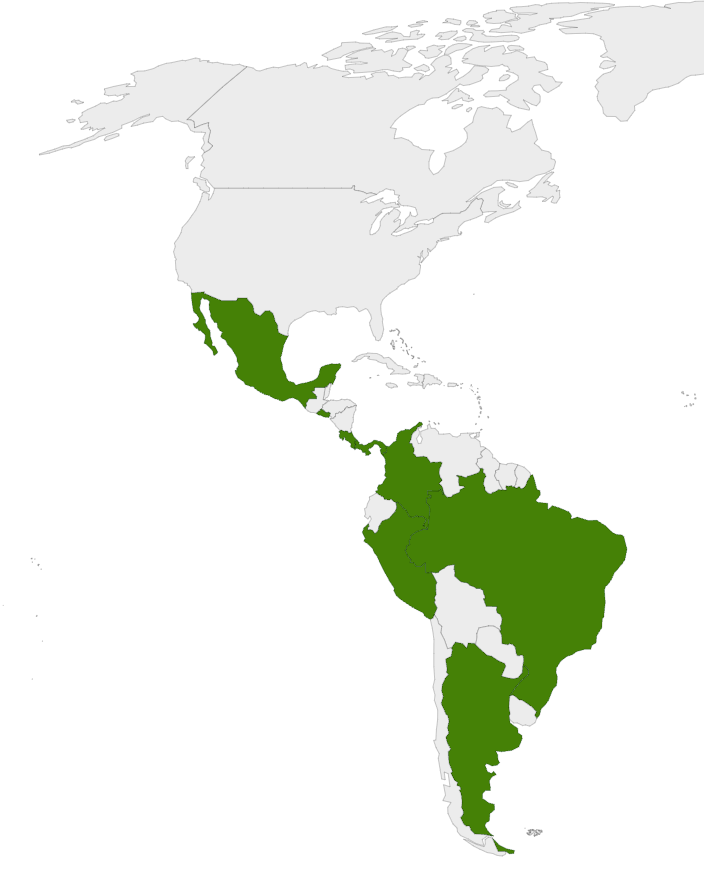
\includegraphics[width=0.5\textwidth]{Images/npdb-map.png}
        \caption{Representación de un grafo molecular de la estructura química de la aspirina (acído acetil salicílico)}
        \label{fig:np-graph-representation}
    \end{figure}


\section{Integraci\'on de datos}

\subsection{Evolución de las definiciones de integración de datos}

La integración de datos comenzó a ser objeto de estudio a finales de la década de
1970. Este interés surgió debido a la proliferación de las bases de datos dentro de las organizaciones,
lo que generó la necesidad de contar con sistemas que ofrecieran flexibilidad en su gestión, 
facilidades para la compartición de información y un adecuado nivel de autonomía.

En este contexto surge el concepto de \textit{base de datos descentralizada} \cite{mcleod1980federated}, la cual es una
colección de información que puede ser:
\begin{itemize}
    \item \textbf{Lógicamente descentralizada}: La base de datos se divide en componentes con el objetivo
    de permitir un control independiente sobre cada uno de ellos. Este control incluye la capacidad de definir
    el significado y la estructura lógica de los datos, los métodos de acceso disponibles para los usuarios y las
    modalidades mediante las cuales los usuarios pueden visualizar la información.
    \item \textbf{Físicamente distribuida}: Los datos se almacenan en nodos de una red o en una arquitectura alternativa de
    sistemas computacionales interconectados.
\end{itemize}

Hasta 1980 el principal enfoque hacia base de datos descentralizadas eran las
\textit{bases de datos distribuidas} \cite{mcleod1980federated}. En este enfoque se define un esquema lógico
único que describe los datos en cada una de las bases de datos que conforman el sistema distribuido. Mientras que la implementación
física de la base de datos se distribuye entre las computadoras de una red. Sin embargo,
la centralización lógica característica de este enfoque presenta muchos problemas prácticos, como la
imposibilidad de optimizar el almacenamiento de datos para cada nodo de la red y la vulnerabilidad del sistema frente a fallos en alguna de las computadoras.


Motivados por las limitaciones de las bases de datos distribuidas, McLeod y Heimbigner \cite{mcleod1980federated} propusieron, en 1980, una nueva
arquitectura de base de datos descentralizada que no solo permitiera la distribución física de los datos, sino también
la descentralización lógica de sus componentes. Esta arquitectura se denominó \textit{base de datos federada}, la cual:

\begin{itemize}
    \item Consiste en un conjunto de componentes lógicos, cada uno de los cuales posee su propio esquema conceptual/lógico.
    \item Los componentes están interrelacionados, pero son independientes entre sí. Generalmente, cada componente de una federación
    corresponde a una colección de información requerida por una apliación específica o un conjunto de aplicaciones
    estrechamente relacionadas.
    \item Los componentes de una federación están interrelacionados a través de uno o más esquemas federales, los cuales definen 
    los elementos comunes entre los distintos componentes. Estos esquemas se utilizan para especificar la información  que puede ser compartida
    entre los componentes, funcionando como interfaz para la comunicación entre estos.
\end{itemize}

La primera solución computacional para la integración de datos fue Multibase \cite{smith1981multibase} descrito como \textit{``un sistema de software
diseñado para la integración de bases de datos distribuidas heterogéneas preexistentes''} que responde a la necesidad
de ``\textit{una base de datos integrada descrita por un esquema único, a partir del cual se expresan todos los accesos a los datos que son
procesados en las unidades lógicas independientes}''.
% 1980 - 1989

    Entre los años 1984 y 2000, los esfuerzos se centraron en la integración de bases de datos relacionales, las cuales
    se encontraban en pleno auge.  
    En este contexto múltiples autores conceptualizaron el problema como
    la generalización de los esquemas locales mediante la creación de un esquema global que los unificara y controlara el acceso a estos.
        \begin{itemize}
            \item 
            %McLeod y Heimbigner (1985) \cite{McLeod1985} diseñaron una arquitectura de \textit{base de datos integrada} formada a partir de
            %un conjunto de bases de datos heterogéneas y autónomas, y señalaron que 
            \textit{``Para formar una base de datos integrada, se debe introducir un nuevo esquema conceptual global/virtual,
            el cual describa la información de las bases de datos que lo componen; las operaciones de acceso y manipulación
            de datos se deben llevar a cabo a través de este nuevo esquema conceptual''} McLeod y Heimbigner (1985) \cite{McLeod1985}.

            \item 
            %Batini et al. (1986) \cite{Batini1986} definió el problema de \textit{integración de bases de datos} como 
           \textit{``La integración de bases de datos es la necesidad de un esquema global integrado, diseñado a partir de los esquemas locales, el cual se refiera a bases de datos existentes''} Batini et al. (1986) \cite{Batini1986}.

            \item \textit{``Dado un conjunto de esquemas locales, crear un esquema integrado tal que cada esquema local pueda ser considerado como una vista
            del esquema integrado''} Breitbart (1990) \cite{breitbart1990multidatabase}.
           
        \end{itemize}

Por otro lado, durante este mismo periodo varios autores empezaron a generalizar el concepto
al abstraerse de la tecnología detrás de las fuentes de datos y enfocándose en los propios datos y su
semántica.
\begin{itemize}
    \item \textit{``La integración de datos asegura que los datos tengan el mismo significado y utilidad para los usuarios a través del tiempo, haciendo que los datos en distintos sistemas o bases de datos sean consistentes o logicamente compatibles.''} Martin, J. (1986) \cite{martin1986information}.
    
    \item \textit{``La integración de datos se refiere a la creación de una vista integrada a partir de datos aparentemente
    incompatibles, generalmente obtenidos de diversas fuentes''} Deen et al. (1987) \cite{deen1987data}.
   
    \item \textit{``La utilización de definiciones de atributos y reglas comunes a lo largo de distintas partes
    de la organización''} Goodhue et al. (1992) \cite{goodhue1992impact}.
\end{itemize}


Durante la expansión de los servicios web en la década del 2000 se acrecentó el interés por la integración
de datos semiestructuradas y no estructurados, debido al surgimiento de nuevos formatos de transmisión
de datos como XML \cite{bourret1999xml}. Además, surge un nuevo enfoque de integración, planteando asegurar la interoperabilidad
de sistemas de información mediante la implementación de las nuevas interfaces de comunicación ofrecidas por los servicios web como SOAP, WSDL y UDDI \cite{curbera2002soap}.

\begin{itemize}
    \item \textit{``Al proveer interfaces estándares, los servicios web puede ser considerados como un paradigma de 
    programación para extraer e integrar datos a partir de sistemas de información heterogéneos''} Hansen et al. (2002) \cite{hansen2002data}.
    
    \item \textit{``La integración de datos es un desafío enfrentado por las aplicaciones que necesitan
    ejecutar consultas entre múltiples fuentes de datos autónomas y heterogéneas''} Halevy et al. (2006) \cite{halevy2006data}. 
    
    \item \textit{``La integración de múltiples sistemas de información tiene como objetivo combinar distintos sistemas para ofrecer
    al usuario la ilusión de que está interactuando con un único sistema''}  Ziegler y Dittrich (2007) \cite{ziegler2007data}.

\end{itemize}

A partir de 2010 y hasta la fecha los aportes a la definición de la integración de datos se han
centrado en la integración de \textit{Big Data}, \textit{Open Data} e integración dinámica.
Dong y Srivastava (2013) \cite{dong2013big} señalaron que la integración de Big Data difiere de la integración
de datos tradicional en diferentes aspectos:
    \begin{itemize}
        \item \textit{``incluso para un solo dominio, el número de fuentes de datos ha crecido hasta las decenas de miles''}
        \item \textit{``las fuentes de datos son muy dinámicas, debido a que enormes cantidades de nuevos datos recolectados son
        publicados de forma constante''}
        \item \textit{``las fuentes de datos son extremadamente heterogéneas en su estructura''}
    \end{itemize}
Por otro lado, Miller, R. (2018) \cite{miller2018open} propone que gracias al surgimiento de \textit{Open Data} la integración de datos
puede hacerse de forma dinámica durante el proceso de análisis de datos. ``La integración de datos es guiada
por las necesidades del análisis de datos y por tanto, el descubrimiento de datos es realizado para facilitar este análisis.
El análisis de datos requiere el descubrimiento de joins, uniones y agregaciones existentes en los datos de forma
precisa. Un nuevo enfoque llamado descubrimiento de datos orientado a consultas''.

Las definiciones analizadas pueden ser agrupadas en tres corrientes principales influidas
por el contexto histórico y tecnológico:
\begin{itemize}
    \item \textbf{Federación de datos} (1980s y 1990s) conceptualizaban el problema como la creación de una base de datos
    física centralizada con un esquema unificado.
    \item \textbf{Intercambio de datos} (2000s y 2010s): conceptualizaban el problema como el establecimiento de mecanismo
    de comunicación y compartición de datos entre disintos sistemas de información.
    \item \textbf{Orientación a consultas} (2020s): conceptualizan el problema como el proceso de búsqueda e integración
    dinámica de los resultados de consultas obtenidos de un conjunto dinámico de fuentes de datos.
\end{itemize}
La figura \ref{fig:data-integration-timeline} presenta una breve resumen de la evolución histórica de las corrientes
conceptuales de la integración de datos.


\begin{figure}[h!]
    \centering
    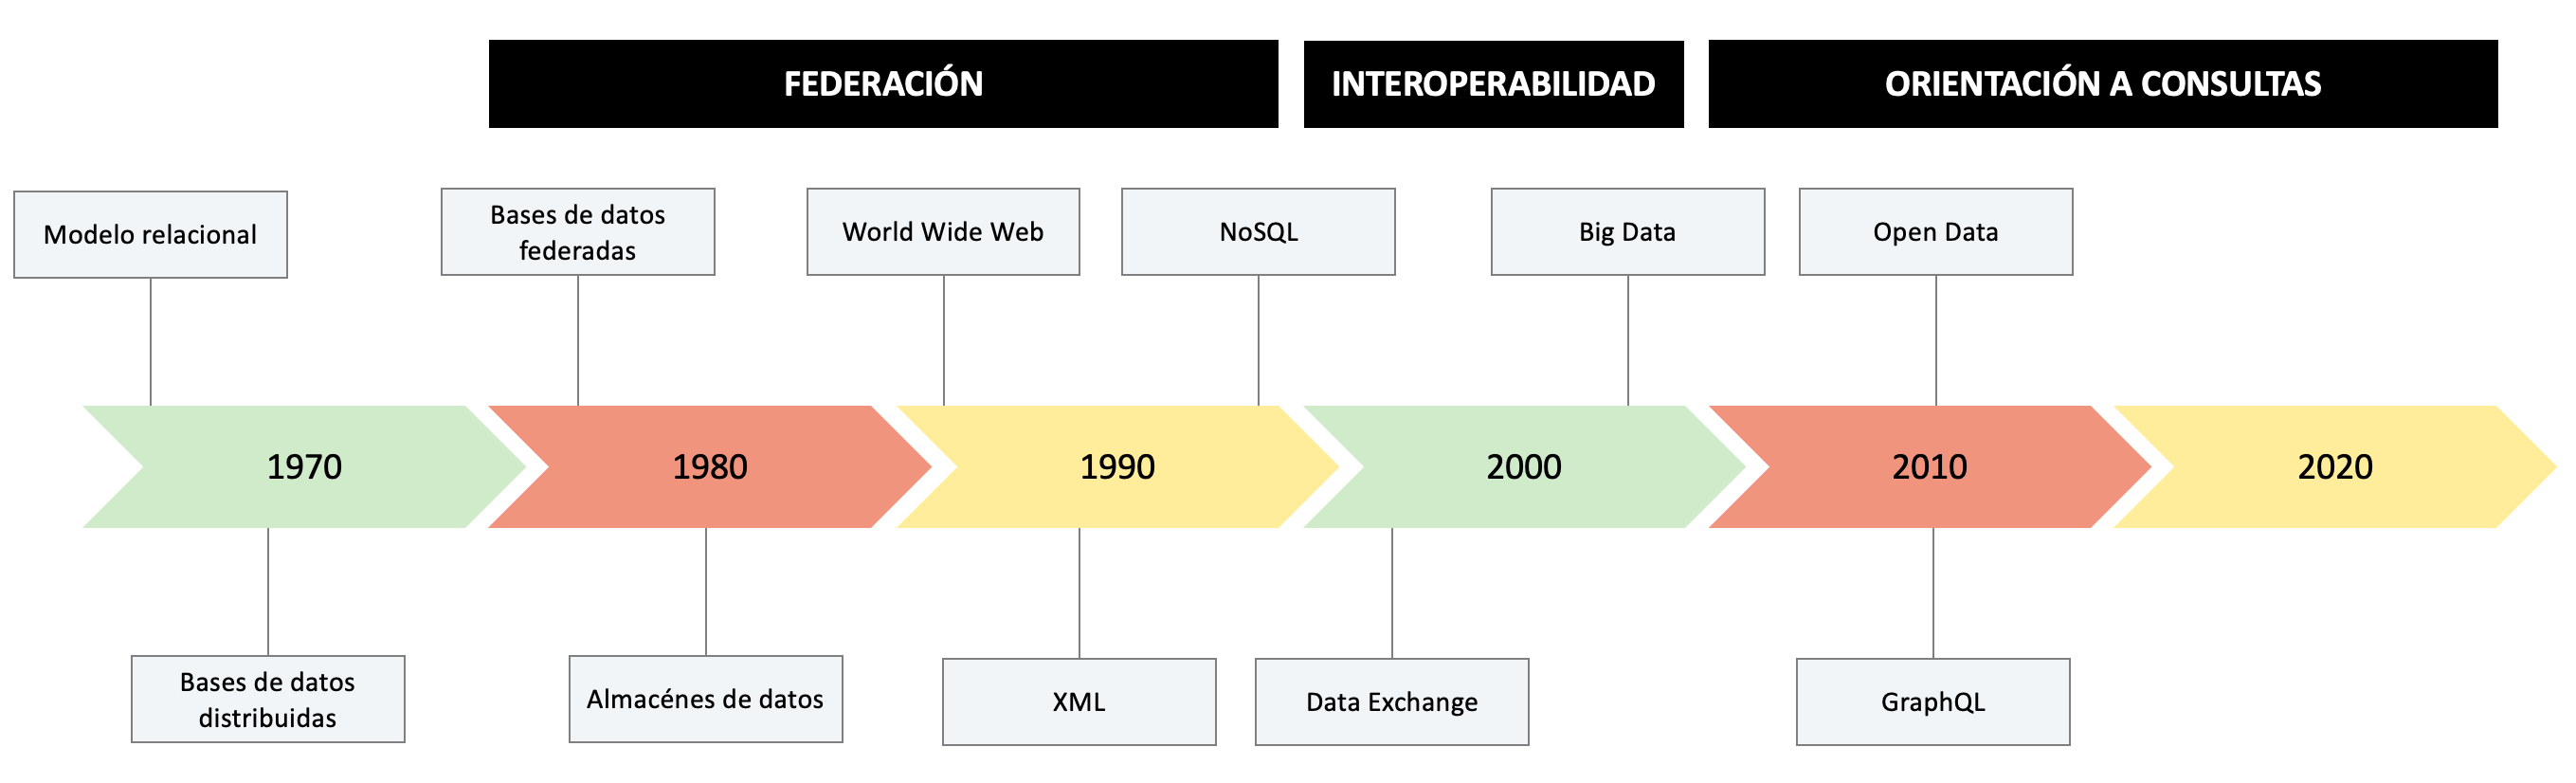
\includegraphics[width=\textwidth]{Images/data-integration-timeline.png}
    \caption{Evolución conceptual de la integración de datos}
    \label{fig:data-integration-timeline}
\end{figure}


A pesar de las visibles diferencias, se pueden identificar elementos clave comunes en estas definiciones, estos son:

\begin{itemize}
    \item \textbf{Consultas}: El objetivo principal de la integración de datos es permitir la ejecución de consultas sobre varios
    sistemas de información o varias fuentes de datos heterogéneas. Además, existen casos donde también resulta de interés poder actualizar las fuentes de datos.

    \item \textbf{N\'umero de objetivos}: La integración de datos se considera un desafío incluso para un pequeño número de objetivos de integración,
     este dasafío solo es exacerbado a medida que el número de objetivos crece. 

    \item \textbf{Heterogeneidad}: La integración de datos usualmente se realiza sobre sistemas desarrollados de manera
    independiente. Como consecuencia estos sistemas son implementados utilizando distintas tecnologías, algunos utilizan sistemas gestores
    de bases de datos, sistemas de gestión de contenido o simplemente archivos en un directorio. Las fuentes de datos subyacentes tendrían distinto
    esquema y metadatos, incluso cuando se utilizan para modelar el mismo dominio. Algunas fuentes de datos pueden almacenar datos estructuradas mientras otras contienen datos semiestructuradas o no estructurados.

    \item \textbf{Autonom\'ia}: Los objetivos de la integración no necesariamente deben pertenecer a una úniqua entidad administrativa,
    e incluso cuando lo hacen, pueden ser mantenidos por diferentes suborganizaciones. Por tanto, no es posible asumir un accesso total
    a los datos o incluso, que este acceso sea ininterrumpido. Además, los sistemas pueden modificar sus patrones de acceso y las fuentes de datos pueden modificar sus esquemas y
    formatos en cualquier momento sin necesidad de notificar a una entidad administrativa.
\end{itemize}

\subsection{Limitaciones de la integración de datos}

    Para abordar de manera efectiva los desafíos que plantea la integración de datos, es fundamental analizar las causas subyacentes que contribuyen a la complejidad de esta tarea. Las limitaciones en la integración de datos son una consecuencia directa de las características intrínsecas de las bases de datos descentralizadas, siendo las más relevantes la heterogeneidad y la autonomía.




    \subsubsection{Limitaciones de infraestructura}

    Las limitaciones de infraestructura se evidencian al intentar que diferentes sistemas, a menudo heterogéneos en términos de tecnología, arquitectura y protocolos, puedan comunicarse de manera consistente. 
    Estas limitaciones suelen estar relacionadas con la falta de interoperabilidad entre plataformas, la diversidad en los modelos de datos, y las discrepancias en los mecanismos de comunicación utilizados por las distintas aplicaciones o sistemas.
    Además, estas dificultades se ven agravadas por la obsolescencia de infraestructuras heredadas (legacy systems), 
    que no fueron diseñadas para integrarse fácilmente con tecnologías más modernas. 
    
    % La necesidad de establecer conexiones fiables, mantener la coherencia de los datos en tiempo real y minimizar los riesgos de pérdida o corrupción de la información son factores clave que demandan soluciones avanzadas, como el uso de middleware, APIs robustas, y arquitecturas orientadas a servicios (SOA) o basadas en microservicios.
    % Superar estas limitaciones requiere no solo inversiones en infraestructura tecnológica, sino también la implementación de estrategias de gobernanza de datos, capacitación del personal, y la adopción de herramientas y metodologías que faciliten la integración, como ETL (Extract, Transform, Load), plataformas de integración como servicio (iPaaS) y estándares de interoperabilidad.

    A continuación, se presenta un resumen de los principales obstáculos identificados y analizados en la literatura científica \cite{mcleod1980federated, reddy1994methodology, doan2012principles}.

    \begin{itemize}
        \item \textbf{Interfaces de comunicación}: Los diferentes tipos de sistemas emplean distintos mecanismos de comunicación. 
        Por ejemplo, los sistemas de bases de datos suelen utilizar protocolos propietarios basados en TCP/IP \cite{eddy2022tcp}, lo que requiere el uso de conectores específicos (\textit{drivers}) para cada uno de ellos.
        Los servicios web generalmente emplean APIs REST basadas en HTTP \cite{bishop2022http} para la transferencia de datos, mientras que servidores de archivos pueden utilizar protocolos como FTP \cite{rfc4217ftp}. Por tanto, un sistema
        integrador requiere de la implementación de distintos tipos de conectores de acuerdo a los protocolos de comunicación de las distintas fuentes.
        
        \item \textbf{Modelo de datos}: La diferencia entre modelos de datos se puede traducir en una diferencia a nivel
        de estructura de datos, restricciones de integridad u operaciones. Por ejemplo, en el modelo relacional la única forma
        de representar una interrelación es utilizando una llave foránea, sin embargo, en modelos orientados a documentos una
        interrelación puede ser representada mediante llaves foráneas o embebiendo los documentos relacionados directamente dentro
        del documento principal \cite{mongodb2024embedding}. Estas diferencias provocan que se deban no solo realizar cambios en la
        sintaxis de las consultas sino también en la lógica de acceso a los datos.

        \item \textbf{Lenguajes de consulta}: Incluso entre sistemas gestores de bases de datos que utilizan el mismo modelo
        de datos existen diferencias entre sus lenguajes de consulta de cada uno. Por ejemplo, a pesar de la existencia
        del estándar SQL diferentes sistemas gestores comerciales como Oracle, PostgreSQL, MySQL y SQLServer han realizado
        distintas implementaciones de SQL. Por tanto, se requiere de una traducción a distintos lenguajes de las consultas para
        la integración de datos.

        \item \textbf{Sistemas heredados}: Incluso dentro de un mismo sistema, el paso del tiempo puede generar incompatibilidades 
        como resultado de actualizaciones, cambios en los estándares o en los protocolos de comunicación, 
        así como modificaciones en las estructuras de datos y en las interfaces de programación.
        Además, el soporte limitado, la falta de cortafuegos y protocolos de cifrado, así como la incompatibilidad con las 
        herramientas de seguridad modernas, hacen que los sistemas heredados sean vulnerables a ataques cibernéticos.
    \end{itemize}

    % An enterprise may have multiple DBMSs.  Different organizations within the enterprise may have different requirements and  may select different DBMSs. DBMSs  purchased over a period of time may be  different due to changes in technology. Heterogeneities due to differences in DBMSs  result from differences in data models and  differences at the system level. These are  described below. Each DBMS has an underlying data model used to define data  structures and constraints. Both representation (structure and constraints) and language aspects can lead to heterogeneity.  l Differences in structure: Different  data models provide different structural  primitives [e.g., the information modeled  using a relation (table) in the relational  model may be modeled as a record type  in the CODASYL model]. If the two representations have the same information  content, it is easier to deal with the differences in the structures. For example,  address can be represented as an entity  in one schema and as a composite attribute in another schema. If the information content is not the same, it may be  very difficult to deal with the difference.  As another example, some data models  (notably semantic and object-oriented  models) support generalization (and  property inheritance) whereas others do  not.  l Differences in constraints: Two data  models may support different constraints. For example, the set type in a  CODASYL schema may be partially  modeled as a referential integrity constraint in a relational schema. CODASYL, however, supports insertion and  retention constraints that are not captured by the referential integrity constraint alone. Triggers (or some other  mechanism) must be used in relational  systems to capture such semantics.  l Differences in query languages:  Different languages are used to manipulate data represented in different data  models. Even when two DBMSs support  the same data model, differences in their  query languages (e.g., QUEL and SQL)  or different versions of SQL supported  by two relational DBMSs could contribute to heterogeneity. system aspects of the  DBMSs also lead to heterogeneity. \cite{mcleod1980federated}

    % Data retrieved from two local databases for the same logical data item may be incompatible for the following reasons:  * Different Levels of Accuracy: Different databases may be storing an attribute at dissimilar levels of accuracy. For example, one database may contain the weight of a particular part up to an accuracy of a milligram, whereas another database may specify accuracy only up to a gram [43]. * Asyncronous Updates: Since each database is managed independently, all databases may not update the value simultaneously [481. * Lack of Security: Due to lack of information security at component databases, unauthorized users may have changed the data [491. \cite{reddy1994methodology}

    \subsubsection{Limitaciones l\'ogicas}

    La individualidad es una característica intrínseca de la naturaleza humana,
    como consecuencia distintos grupos de usuarios o diseñadores pueden interpretar y
    abordar los requerimientos de un sistema de información desde distintas perspectivas y enfoques \cite{doan2012principles, halevy2006data}. Por tanto, cuando se integran
    múltiples fuentes de datos la representación de los datos en cada una puede ser muy distinta.
    Estas diferencias en la representación son agrupadas bajo el concepto de \textit{``heterogeneidad lógica''}, la cual se divide en dos categorías principales
    de problemas \cite{hakimpour2001resolving}. A continuación, se presenta un resumen de los principales obstáculos identificados y analizados en la literatura científica \cite{Batini1986, breitbart1986database, breitbart1990multidatabase, reddy1994methodology, halevy2006data, hakimpour2001resolving}.

    La \textit{``heterogeneidad de datos''} se refiere a diferencias en la implementación de definiciones semánticamente equivalentes entre distintas fuentes de datos. 

    \begin{itemize}
        \item \textbf{Tipo de dato}: Ocurre cuando datos idénticos, desde un punto de vista semántico, se representan
        utilizando diferentes tipos de datos. Por ejemplo, una fecha puede expresarse mediante una cadena de texto siguiendo
        el estándar ISO 8601 \cite{iso8601}, como \texttt{``2024-12-16''}, 
        mediante un valor entero siguiendo estándar del tiempo de Unix \cite{unix_time_wiki} (representando el número de segundos desde el 1 de enero de 1970), o mediante un objeto específico para la gestión de fechas.
        \item \textbf{Precisión}: Esta incompatibilidad surge cuando el mismo atributo de una entidad es almacenado utilizando 
        diferentes unidades de medida o niveles de precisión, como el número de lugares decimales o el número de componentes en la hora. Por ejemplo, un atributo \texttt{longitud}
        puede ser representado en una base de datos en centímetros (cm), mientras que en otra base de datos el mismo atributo se almacena en milímetros (mm).
        \item \textbf{Formato}: Algunos conceptos pueden representarse utilizando diferentes formatos. Un ejemplo claro es el caso de la hora. 
        El estándar ISO 8601 establece múltiples formatos válidos para representar horas, permitiendo diversas configuraciones incluso al mismo nivel
        de precisón (\texttt{``21:47:55Z''} y \texttt{``T214755Z''}).
    \end{itemize}

    La ``heterogeneidad semántica'' se refiere a diferencias o similaridades en el significado de las definiciones del esquema.

    \begin{itemize}
        \item \textbf{Conflictos de nombre}: Los esquemas en distintos modelos de datos utilizan nombres para describir los conjuntos
        de entidades y sus atributos. Sin embargo, las profesionales de diferentes áreas, incluso dentro de una misma organización, pueden emplear
        terminologías completamente distintas debido a la existencia de acrónimos y
        términos sinónimos. Por tanto, es necesario resolver
        los conflictos que ocurren cuando conceptos semánticamente equivalentes son nombrados de manera
        diferente o cuando conceptos semánticamente distintos reciben el mismo nombre.
        \item \textbf{Conflictos de llave}: En distintos esquemas de datos pueden asignarse diferentes llaves a un mismo concepto. Por ejemplo, para
        el conjunto de entidades \texttt{Cliente}, atributos como \texttt{CI} (Carné de identidad) o \texttt{Email} pueden ser utilizados como llave
        en fuentes de datos distintas.
        \item \textbf{Conflictos de interrelación}: La cardinalidad o el grado de una misma interrelación varía en diferentes fuentes de datos. 
        Por ejemplo, una interrelación entre \texttt{Clientes} y \texttt{Pedidos} puede tener una cardinalidad diferente en dos fuentes de datos. 
        En una, esta relación puede ser de uno a muchos (1:m) (un cliente puede realizar múltiples pedidos, el pedido está asociado a un único cliente), 
        mientras que en otra base de datos, la misma interrelación podría tener una cardinalidad de 
        muchos a muchos (m:m) (un cliente puede realizar varios pedidos y cada pedido puede estar vinculado a múltiples clientes).
        \item \textbf{Atributos faltantes}: Un mismo concepto puede ser representado mediante diferentes atributos, dependiendo de los intereses y objetivos de las organizaciones que diseñan su esquema de datos. 
        Las distintas organizaciones pueden priorizar diferentes aspectos o medidas del concepto, lo que lleva a la creación de atributos específicos que varían en términos de definición o granularidad. 
        Por ejemplo, un concepto como \texttt{precio} puede ser representado por un atributo que incluye solo el valor numérico, o puede desglosarse en atributos adicionales como \texttt{precio base}, \texttt{impuestos} y \texttt{descuentos},
        dependiendo de las necesidades de cada organización.
    \end{itemize}


    % In the design process, different user groups  or designers adopt their own viewpoints in  modeling the same objects in the application domain.



    % It quickly became clear that one of the major bottlenecks in setting up a data integration application is the effort required to create the source descriptions, and more specifically, writing the semantic mappings between the sources and the mediated schema. Writing such mappings (and maintaining them) required database expertise (to express them in a formal language) and business knowledge (to understand the meaning of the schemas being mapped). \cite{halevy2006data}
    % The work on automated schema mapping was based on the following foundations. First, the research explored techniques to map between schemas based on clues that can be obtained from the schemas themselves, such as linguistic similarities between schema elements and overlaps in data values or data types of columns. Second, based on the observation that none of the above techniques is foolproof, the next development involved systems that combined a set of individual techniques to create mappings [31, 32]. Finally, one of the key observations was that schema mapping tasks are often repetitive. For example, in data integration we map multiple schemas in the same domain to the same mediated schema. Hence, we could use Machine Learning techniques that consider the manually created schema mappings as training data, and generalize from them to predict mappings between unseen schemas. As we describe in Section 4, these techniques are in commercial use today and are providing important benefits in the settings in which they are employed.

    % We distinguish two types of heterogeneity here: data heterogeneity and semantic heterogeneity. 
    % Data heterogeneity refers to differences among local definitions, such as attribute types, formats, or precision. These differences can be easily resolved.
    %  Semantic heterogeneity refers to differences or similarities in the meaning of local data. For example, two schema elements in two local data sources can have the same intended meaning, but different names. 
    %  Thus, during integration, it should be realized that these two elements actually refer to the same concept. 
    %  Alternatively, two schema elements in two data sources might be named identically, while their intended meanings are incompatible. 
    %  Hence, these elements should be treated as different things during integration. 
    %  As a consequence, adequate and meaningful data integration relies on the detection of discrepancies and similarities between schema elements. 
    %  Thus, semantics of data must be taken into account during integration. Semantics is the interpretation people attribute to data (i.e., relating data to what they represent) according to their understanding of the world. 
    %  Different interpretations of data causes semantic heterogeneity. In the database domain, semantics refers to the meaning of schema elements (e.g., classes, attributes and methods). Often, it is used in contrast with syntax, by which we refer to the definition of the structure of schema elements. \cite{hakimpour2001resolving}


    % In the heterogeneous environment one of the major problems in schema integration is to resolve data inconsistencies that may exist in different data sources for semantically identical data. The most significant problems of such nature are as follows.  1. resolution of naming conventions and naming conflicts that occur when semantically identical data items are named differently or semantically different data items are named identically.  2. resolution of data representation conflicts that occur when semantically identical data items are represented differently in different data sources (for example, data represented as a character string in one database maybe represented as a real number in the other database).  3. resolution of differences in data structures in different data sources.  4. resolution of data sealing conflicts that occur when semantically identical data items stored in different  databases using different units of measure.  5. resolution of missing or conflicting data values that occur when semantically identical data items may have some attribute values different or missing in some data  SOUrCeS. \cite{breitbart1990multidatabase}


    % Type Conflicts. These arise when the  same concept is represented by different modeling constructs in different  schemas. This is the case when, for  example, a class of objects is represented as an entity in one schema and  as an attribute in another schema.  (2) Dependency Conflicts. These arise  when a group of concepts are related  among themselves with different dependencies in different schemas. For  example, the relationship Marriage between Man and Woman is 1: 1 in one  schema, but m : n in another accounting  for a marriage history.  (3) Key Conflicts. Different keys are assigned to the same concept in different  schemas. For example, SS and Empid may be the keys of Employee in two  component schemas.  (4) Behavioral Conflicts. These arise when  different insertion/deletion policies are  associated with the same class of objects in distinct schemas. For example,  in one schema a department may be  allowed to exist without employees,  whereas in another, deleting the last  employee associated with,a department  leads to the deletion of the department  itself. Note that these conflicts may  arise only when the data model allows  for the representation of behavioral  properties of objects. \cite{Batini1986}


    % resolution of naming conflicts, which typically involves either semantically equivalent data items named differently in different databases, or semantically different data items which have the same name in different databases;  - resolution of data representation conflicts for the same data item in different databases. For example, well depth in the INQUIRE database could be defined as a character data type, while in the IMS database it is defined as real;  - resolution of data scaling conflicts, when the same data item is stored in different databases using different units of measure. For example, well depth in one database is measured in meters and in the other one in feet;  - resolution of data structure conflicts caused by using various data models by different DBMS's;  - resolution of data inconsistencies for the same data item residing in several databases. \cite{breitbart1986database}


    % Semantic Incompatibilities  Naming Conflicts: In any data model, the schemata incorporate names for various entities/objects represented by them. Since these schemata are designed independently, the designer of each schema uses his or her own vocabulary to name these objects. Objects in different schemata representing the same real world concept may contain dissimilar names [1], [21, [141, [451, [71, [4] resulting in problems of two types: Homonyms: This inconsistency arises when the same name is used for two different concepts. For example, 'SALARY' may mean weekly salary in one database, and monthly salary in another.  - Synonyms: This type of naming conflict arises when the same concept is identified by two or more names. For example, the term 'DOMESTICCUSTOMER' in one database may refer to the same concept as the term 'BUYERS' in another database.  Note that homonyms and synonyms can only be detected by external specification. Type Conflicts: These conflicts arise when the same concept is represented by different coding constructs in different schemata [1]. For example, an object may be represented as an entity in one schema and as an attribute in another schema. Key Conflicts: Different keys may be assigned to the same concept in different schemata [15], [46]. For example, ss and EMP-ID may be keys for employees in two component schemata. * Behavioral Conflicts: These conflicts arise when different insertion/deletion policies are associated with the same class of objects in different schemata [151. For example, in one database, the relation DEPT may exist without having any employee records being associated with it, where as in another database, the deletion of the last employee record may also delete the relation DEPT from the database. * Missing Data: Different attributes may be defined for the same concept in different schemata [47]. For example, EMPI(SSN, NAME, AGE) and EMP2(SSN, NAME, ADDRESS) may represent the same concept in two database schemata. Attribute 'AGE' is missing in EMP2, and attribute 'ADDRESS' is missing in EMPI.  * Levels of Abstraction: This incompatibility is encountered when information about an entity is stored at dissimilar levels of detail in two databases [131. For example, 'LABOR-COST' and 'MATERIAL-COST' may be stored separately in one database and combined together as 'TOTAL-COST' in a second database.  * Identification of Related Concepts: For concepts in the component schemata that are not the same but are related, one needs to discover all the inter-schema properties that relate to them. For example, two entities belonging to two different databases may not be equivalent but one entity may be a generalization of the other entity. * Scaling Conflicts: This incompatibility arises when the same attribute of an entity is stored in dissimilar units in different databases [141. For example, the attribute 'LENGTH' of an entity may be stored in terms of centimeters in one database and as inches in another database. \cite{reddy1994methodology}


    \subsubsection{Limitaciones administrativas}

    Si bien la autonomía de las fuentes de datos ofrece diversas ventajas, también conlleva una serie de consecuencias negativas, principalmente relacionadas con la necesidad de armonizar políticas organizacionales y establecer mecanismos efectivos de comunicación entre distintos equipos de personas \cite{miller2018open, mcleod1980federated}.

    \begin{itemize}
        \item \textbf{Acceso}: El acceso a ciertos datos está condicionado por múltiples factores, que incluyen aspectos organizacionales, legales y contractuales. En primer lugar, las políticas internas de las organizaciones propietarias de las fuentes de datos suelen estar orientadas a mantener el control sobre sus activos de información. Esto significa que las organizaciones solo comparten sus datos con terceros bajo estrictas condiciones que aseguren la preservación de dicho control, como la implementación de acuerdos de confidencialidad, políticas de acceso restringido y mecanismos de trazabilidad.
        En segundo lugar, existen regulaciones legales y normativas de protección de datos que imponen restricciones específicas sobre el acceso y uso de información personal. Ejemplos representativos incluyen el Reglamento General de Protección de Datos (GDPR) en la Unión Europea y la Ley de Portabilidad y Responsabilidad del Seguro Médico (HIPAA) en los Estados Unidos. Estas leyes limitan el tratamiento y la transferencia de datos personales, estableciendo principios como el consentimiento explícito del usuario, la minimización de datos y la necesidad de garantizar medidas de seguridad adecuadas. El incumplimiento de estas regulaciones puede acarrear sanciones legales severas, lo que obliga a las organizaciones a implementar mecanismos de cumplimiento que restringen el acceso a información sensible.
        Finalmente, las licencias de uso de los datos representan otra barrera significativa en el acceso y la integración de fuentes de información. Dependiendo del tipo de licencia, pueden establecerse restricciones sobre la reutilización, modificación, distribución o explotación comercial de los datos. Por ejemplo, ciertas licencias abiertas, como Creative Commons, permiten un uso más flexible, mientras que licencias propietarias restringen su utilización a términos específicos acordados entre las partes.
        \item \textbf{Comunicación}: Una fuente de datos puede llevar a cabo actualizaciones o modificaciones en su estructura, formato o protocolos de acceso que comprometan la interoperabilidad con otros sistemas dependientes. Estas actualizaciones pueden ser realizadas sin una adecuada comunicación o coordinación con los sistemas y aplicaciones que consumen los datos, lo que puede provocar una serie de problemas técnicos y operativos.
    \end{itemize}


\subsection{Arquitecturas de sistemas de integraci\'on de datos}

\subsubsection{Componentes de una arquitectura de integración de datos}

A partir del análisis de la literatura científica , se han identificado y recopilado los componentes fundamentales que constituyen las arquitecturas de integración de datos.

\begin{itemize}
    \item \textbf{Esquema mediador}: The mediated schema is built for the data integration application and contains only the aspects of the domain that are relevant to the application. As such, it does not necessarily contain all the attributes we see in the sources, but only a subset of them. In the virtual approach the mediated schema is not meant to store any data. It is purely a logical schema that is used for posing queries by the users (or applications) employing the data integration system.
    \item \textbf{Fuentes de datos}: Data sources can vary on many dimensions, such as the data model underlying them and the kinds of queries they support. Examples of structured sources include database systems with SQL capabilities, XML databases with an XQuery interface, and sources behind Web forms that support a limited set of queries (corresponding to the valid combinations of inputs to its fields). In some cases, the source can be an actual application that is driven by a database, such as an accounting system. In such a case, a query to the data source may actually involve an application processing some data stored in the source.
    \item \textbf{Decoradores}: and their role is to send queries to a data source, receive answers, and possibly apply some basic transformations on the answer. For example, a wrapper to a Web form source would accept a query and translate it into the appropriate HTTP request with a URL that poses the query on the source. When the answer comes back in the form of an HTML file, the wrapper would extract the tuples from the HTML file.
    \item \textbf{Metadatos}: the glue that connects the mediated schema and the schemas of the sources. These descriptions specify the properties of the sources that the system needs to know in order to use their data.
    \item \textbf{Mapeos semánticos}: which relate the schemata of the data sources to the mediated schema. The semantic mappings specify how attributes in the sources correspond to attributes in the mediated schema (when such correspondences exist), and how the different groupings of attributes into tables are resolved. In addition, the semantic mappings specify how to resolve differences in how data values are specified in different sources. It is important to emphasize that the virtual data integration architecture only requires specifying mappings between the data sources and the mediated schema and not between every pair of data sources. Hence, the number of mappings we specify is the same as the number of sources and not the square of that number.
\end{itemize}

\subsubsection{Arquitecturas de integración de datos física}

\paragraph{Data warehouse\newline}

El término \textit{data warehouse} fue introducido a finales de la década de 1980 por los investigadores Barry Devlin y Paul Murphy en
su propuesta de arquitectura para asegurar el flujo de datos hacia los ambientes de toma de decisión \cite{Devlin1988AnAF}. En 1992 Inmon \cite{inmon1992building} definió formalmente
el data warehouse como \textit{``una colección de datos integrada, orientada a sujetos, variante en el tiempo y no volátil, utilizada como soporte para los procesos de toma de decisión''}.
Por su parte, Raph Kimball propuso en 1996 que \textit{``Un data warehouse es un sistema que extrae, limpia, conforma y entrega los datos fuentes a un almacén de datos dimensional que soporta la ejecución de consultas y el análisis con el propósito de la toma de decisiones''} \cite{kimball1996data}.

La architectura básica de un data warehouse se encuentra dividida en tres capas conceptuales \cite{kimball2013data,jameel2022analyses,nambiar2022overview} (véase figura \ref{fig:dw-architecture}):

\begin{itemize}
    \item \textbf{Capa de datos en tiempo real}: Incluye las fuentes de datos estructurados, 
    generalmente provenientes de sistemas transaccionales con distintos esquemas. 
    Asimismo, contiene la llamada zona de preparación (\textit{staging zone}), 
    donde los datos extraídos de estas fuentes se almacenan en su estado original 
    para facilitar un procesamiento más eficiente.
    \item \textbf{Capa de datos reconciliados}: 
    En esta capa, los datos se integran en un esquema lógico global, 
    diseñado siguiend los principios de normalización para garantizar la consistencia de la información. 
    Posteriormente, los datos correspondientes a una rama específica del negocio se denormalizan 
    y se almacenan en un data mart para su utilización.
    Según Kimball, R. (2013) \textit{``un data mart presenta los datos producidos por un proceso del negocio''} \cite{kimball2013data}.
Este sistema de almacenamiento 
estructura e integra una pequeña parte de los datos,
específica de una unidad del negocio (por ejemplo, un departamento),
que la empresa almacena en un sistema de almacenamiento más grande.
    \item \textbf{Capa de datos derivados}: Esta capa comprende los datos generados
    a partir del procesamiento de los datos derivados utilizando diversas herramientas de extracción de conocimiento.
\end{itemize}

\begin{figure}[h!]
    \centering
    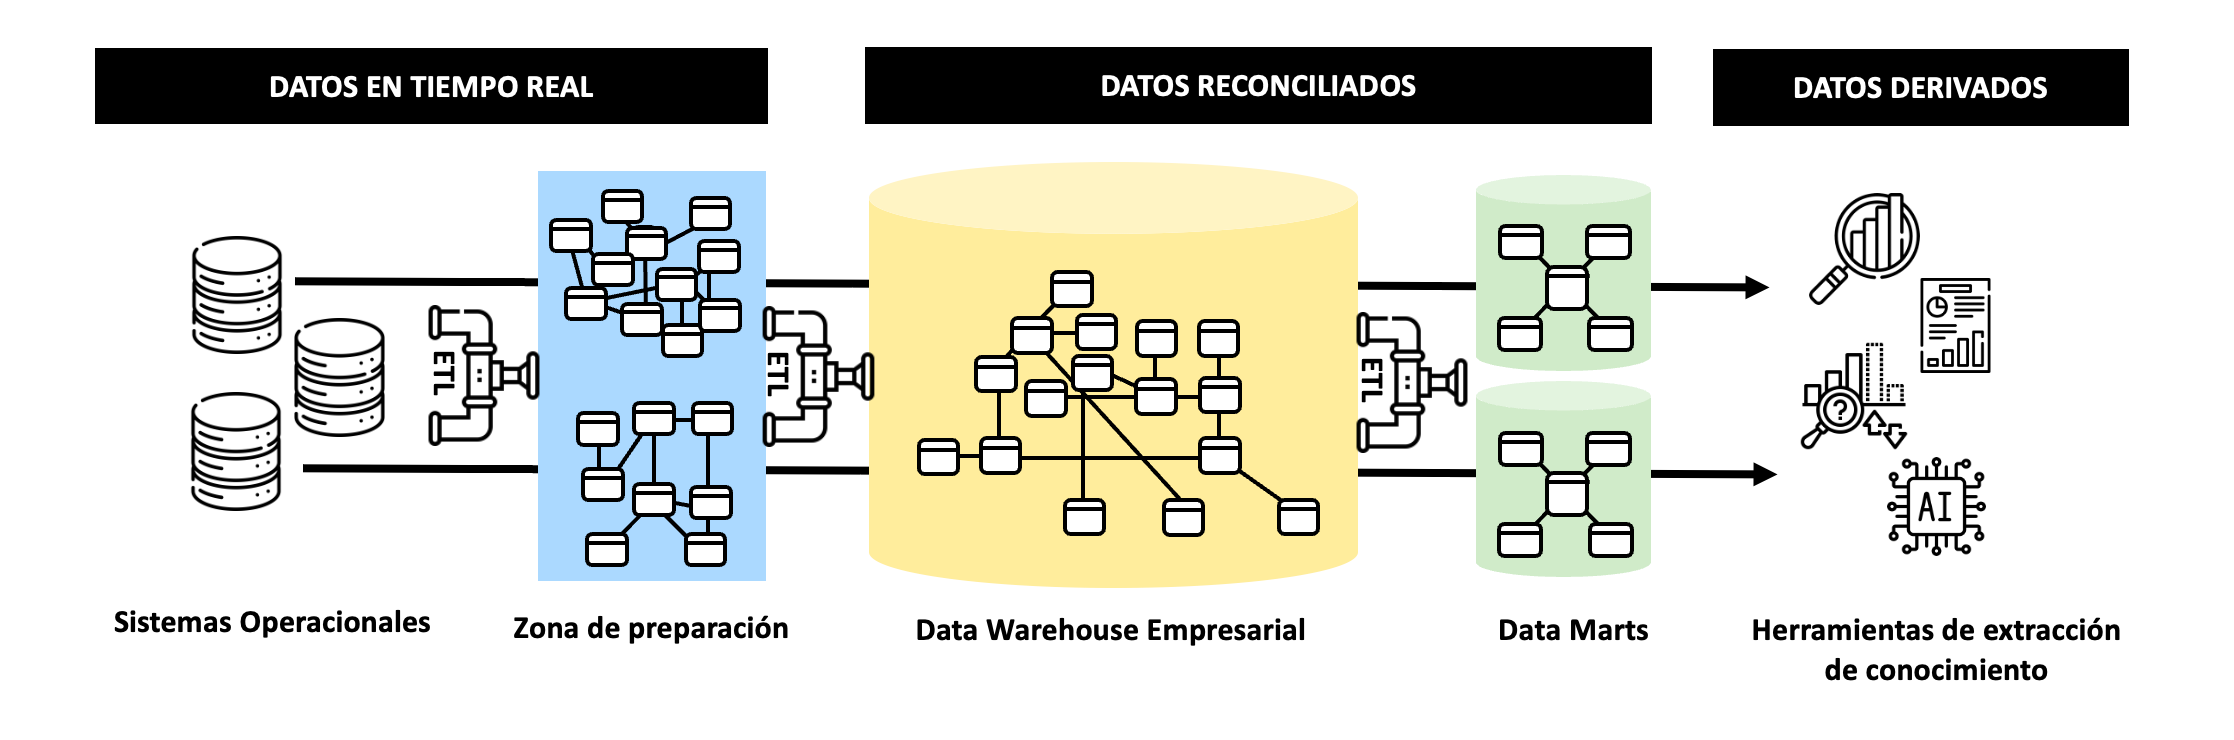
\includegraphics[width=\textwidth]{Images/dw-architecture.png}
    \caption{Arquitectura básica de un \textit{data warehouse}}
    \label{fig:dw-architecture}
\end{figure}


\paragraph{Data lake\newline}

El concepto de \textit{data lake} introducido por Dixon \cite{dixon2010lake} en 2010 como una solución a las limitaciones del \textit{data mart}, que a diferencia de este
\'ultimo se considera como un sistema de almacenamiento para datos heterogéneos y no procesados obtenidos de múltiples fuentes.

La tecnología utilizada para la implementación de los primeros data lakes fue Apache Hadoop \cite{hadoop} que,
gracias a la utilización del formato de almacenamiento de datos Apache Parquet \cite{parquet},
permitía el almacenamiento,
procesamiento y exploración de datos brutos dentro de una organización a bajo costo.
Debido a esto, una parte de la literatura \cite{o2014embedding,fang2015managing} asoció el concepto de \textit{data lake} con la tecnología utilizada para implementarlo, 
sin embargo, esta corriente fue sustituída a medida que la implementación de los data lakes
se asoció cada vez más con soluciones propietarias basadas en la nube y la utilización de tecnologías NoSQL \cite{sirosh2016lake}.

Por otro lado, varios autores [\cite*{mathis2017data, khine2018data,couto2019mapping}] llegaron al consenso de que un data lake podía
ser considerado como \textit{``un repositorio central de datos, almacenados en un formato arbitrario y sin un esquema definido, para futuros análisis''}. Sin embargo,
esta definición omite algunas de las características del almacenamiento de los datos en el data lake, por tanto Madera y Laurent (2016) \cite{madera2016next} señalaron que
\textit{``Un data lake es una vista lógica de todas las fuentes de datos o conjuntos de datos, en su formato original, accesibles solo a
los cietíficos de datos y estadistas para realizar análisis''}, complementando esta definición con las siguientes características:
\begin{itemize}
    \item La calidad de los datos es asegurada utilizando metadatos
    \item El acceso es controlado por herramientas de gobernación de políticas de datos
    \item Su uso es limitado a científicos de datos y estadistas 
    \item Integra todo tipo de datos en distintos formatos
    \item Tiene un diseño lógico y físico
\end{itemize}
Este concepto limita los usuarios a solamente especialista de datos y carece de la noción de escalabilidad. Para
solucionar estas carencias, Sawadomo y Darmont (2021) \cite{sawadogo2021data} proveyeron la siguiente
definicion \textit{``Un data lake es un sistema escalable de almacenamiento y análisis de datos de cualquier tipo en su formato original,
el cual es utilizado principalmente por especialistas de datos para la extracción de conocimiento''} y complementaron su definción con las siguientes
características:
\begin{itemize}
    \item Contiene un catálogo de metadatos que asegura la calidad de datos
    \item Utiliza herramientas de políticas de gobernación de datos
    \item Es accesible a varios tipos de usuarios 
    \item Integra cualquier tipo de datos en sus formatos originales
    \item Tiene un diseño lógico y físico
    \item Es escalable en términos de almacenamiento y procesamiento
\end{itemize}

Las revisiones [\cite*{giebler2019leveraging,ravat2019data}] de las arquitecturas de data lakes usualmente las agrupan en dos tipos: arquitectura de estanques y la arquitectura de zonas.

La arquitectura de estanques fue diseñada por Inmon como un conjunto de estanques de datos \cite{inmon2016data}, donde cada estanque es una
subdivisión del data lake que se encarga de un tipo de datos específico. De acuerdo a las especificaciones de Inmon, cada
estanque está asociado a un tipo de almacenamiento especializado, un procesamiento de datos específico y un servicio para los análisis
relevantes para el tipo de datos. Esta arquitectura es usualmente compuesta por cinco estanques (véase figura \ref{fig:pond-architecture}):

\begin{enumerate}
    \item \textbf{Estanque de datos brutos}: se encarga de procesar los nuevos datos ingeridos y se considera una
    zona de tránsito ya que solo se realizan comprobaciones de calidad básica y los datos se transfieren al estanque
    correspondiente de acuerdo a su tipo. Este estanque es el único que no está asociado a ningún tipo de sistema de gestión de metadatos.
    \item \textbf{Estanque de datos analógicos}: los datos almacenados en este estanque se caracterizan por ser mediciones realizadas en altas frecuencias, es decir,
    mediciones generadas en gran volumen y a gran velocidad. Usualmente, se trata de datos semiestructuradas provenientes de dispositivos
    que utilizan Internet de las cosas (IoT, por sus siglas en inglés).
    \item \textbf{Estanque de datos de aplicación}: como su nombre indica estos datos provienen de aplicaciones de software y usualmente son datos
    estructurados provenientes de algún sistema gestor de bases de datos. Estos datos son integrados, transformados y preparados para posteriores
    análisis, Inmon específicamente considera este estanque como un data warehouse.
    \item \textbf{Estanque de datos textuales}: se encarga de almecenar datos no estructurados y texto.
    \item \textbf{Estanque de datos archivados}: almacena los datos que no son actualmente utilizados en los otros estanques, pero que pueden
    ser requeridos en el futuro. Estos datos pueden ser originados desde los estanques de datos analógicos, de aplicación o de texto.
\end{enumerate}


\begin{figure}[h!]
    \centering
    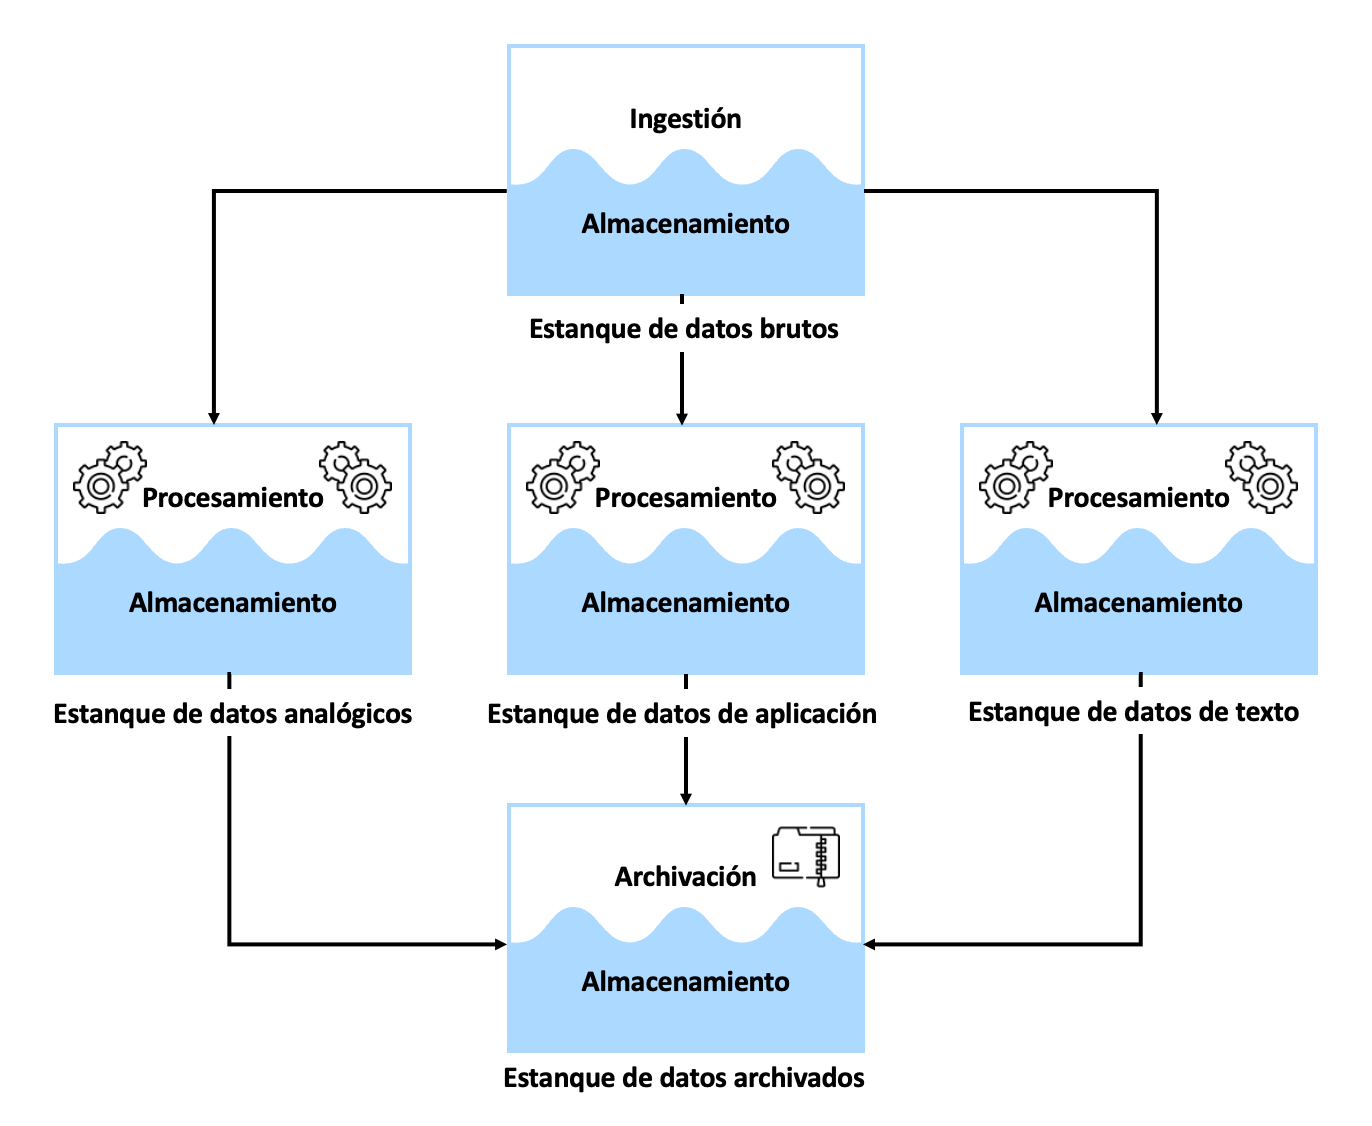
\includegraphics[width=0.7\textwidth]{Images/pond-architecture.png}
    \caption{Arquitectura de estanques para un \textit{data lake}}
    \label{fig:pond-architecture}
\end{figure}


La arquitectura de zonas asigna los datos a una zona de acuerdo a su grado de refinamiento \cite{giebler2019leveraging}. Por ejemplo,
la arquitectura utilizada por Zaloni \cite{sharma2018architecting} se compone de seis zonas (véase figura \ref{fig:zone-architecture}):

\begin{enumerate}
    \item \textbf{Zona de carga}: se encarga de ingerir los nuevos datos y realizar comprobaciones básicas de calidad.
    \item \textbf{Zona de datos brutos}: almacena los datos provenientes de la zona de carga en su formato original.
    \item \textbf{Zona de datos confiables}: almacena los datos una vez han sido depurados y estandarizados.
    \item \textbf{Entorno de escubrimiento}: permite el acceso de los científicos de datos a los datos confiables a través de operaciones de manipulación de datos y APIs. 
    \item \textbf{Zona de consumisión}: permite el acceso los usuarios del negocio y los tomadores de decisiones a los distintos escenarios de análisis mediante paneles de control.
    \item \textbf{Zona de gobernanza}: se encarga de la administración, monitoreo y gobernación de los metadatos, control de la calidad de datos, administración del catálogo de datos y
    la configuración de seguridad y acceso.
\end{enumerate}

\begin{figure}[h!]
    \centering
    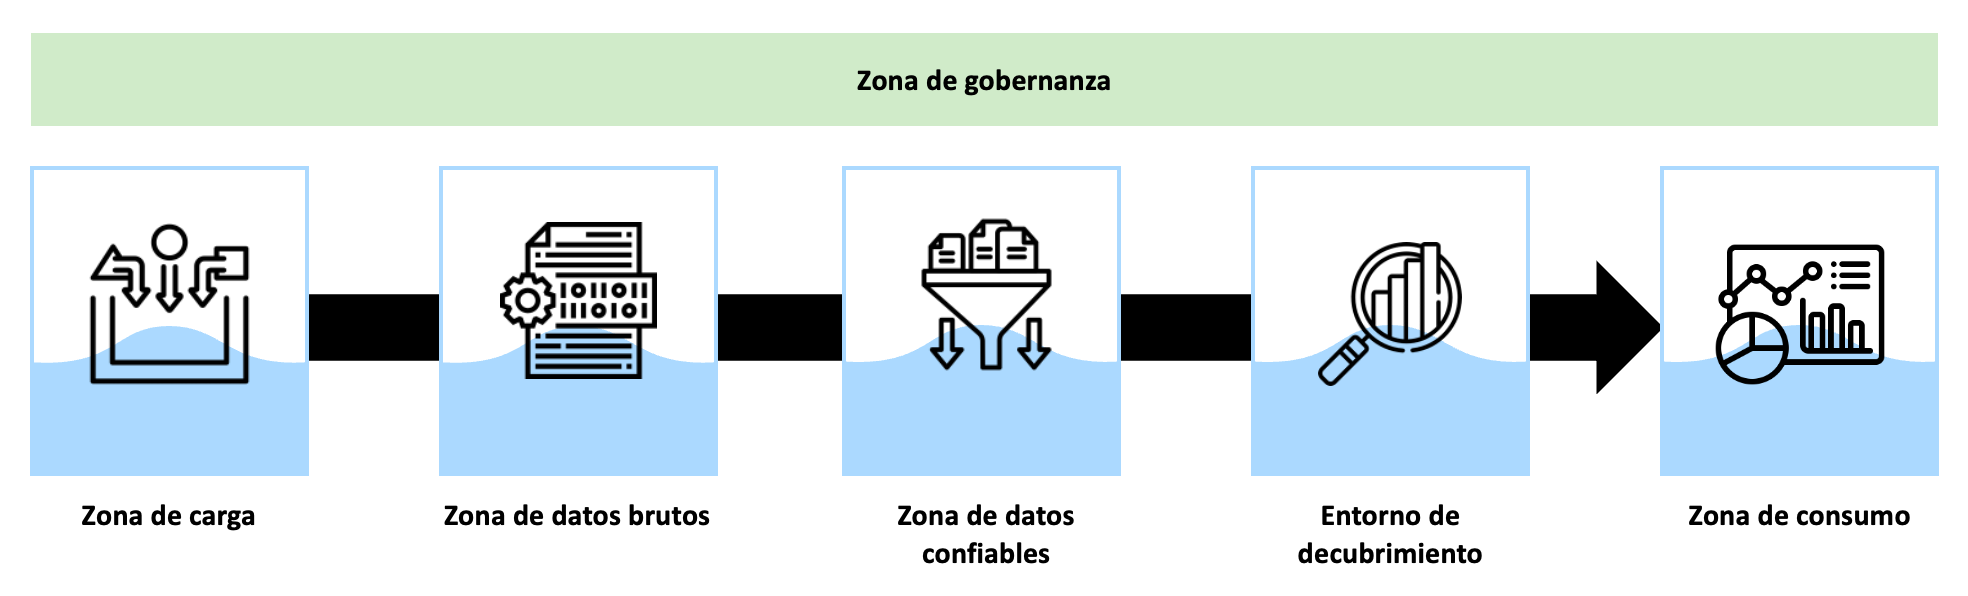
\includegraphics[width=\textwidth]{Images/zone-architecture.png}
    \caption{Arquitectura de zonas para un \textit{data lake}}
    \label{fig:zone-architecture}
\end{figure}


\paragraph{Data lakehouse\newline}

El \textit{data lakehouse} surge como solución a las limitaciones del \textit{data warehouse} y el \textit{data lake}, 
Ambrust et al. (2021) \cite{armbrust2021lakehouse} lo definió como
\textit{`` 
un sistema de gestión de datos basado en un almacenamiento de bajo coste y directamente accesible, 
que también proporciona las funcionalidades y rendimiento de SGBD analíticos, 
como transacciones ACID, versionado de datos, auditoría, indexación, almacenamiento en caché y optimización de consultas. 
De este modo, se combinan las principales ventajas de los data lakes y data warehouses: 
el almacenamiento de bajo coste en un formato abierto accesible por diversos sistemas del primero, y las potentes funciones de gestión y optimización del segundo.
''}

La arquitectura de un data lakehouse (véase figura \ref{fig:dlh-architecture}) se compone de:

\begin{itemize}
    \item \textbf{Data lake}: almacena los datos en un almacén de objetos de bajo coste utilizando un formato de archivo estándar.
    \item \textbf{Capa de metadatos transaccional}: se implementa sobre el almacén de objetos para definir qué objetos forman parte de una versión de una tabla. 
    Esto permite al sistema implementar funcionalidades como las transacciones ACID o el versionado dentro de la capa de metadatos, 
    al tiempo que mantiene el grueso de los datos en un almacenamiento de bajo coste y permite a los clientes leer directamente objetos de este almacén utilizando un formato de archivo estándar en la mayoría de los casos.
    \item \textbf{Catálogo de datos}: define las tablas virtuales que son percibidas por los usuarios.
    \item \textbf{SQL APIs}: el desarrollo de APIs basadas en el estandar de SQL permite la comunicación con la capa de metadatos transaccional.
    \item \textbf{Dataframe APIs}: Las APIs declarativas de DataFrame se implementan  
    para optimizar el rendimiento de las bibliotecas de aprendizaje de máquinas como TensorFlow \cite{tensorflow2015-whitepaper}.
\end{itemize}

\begin{figure}[h!]
    \centering
    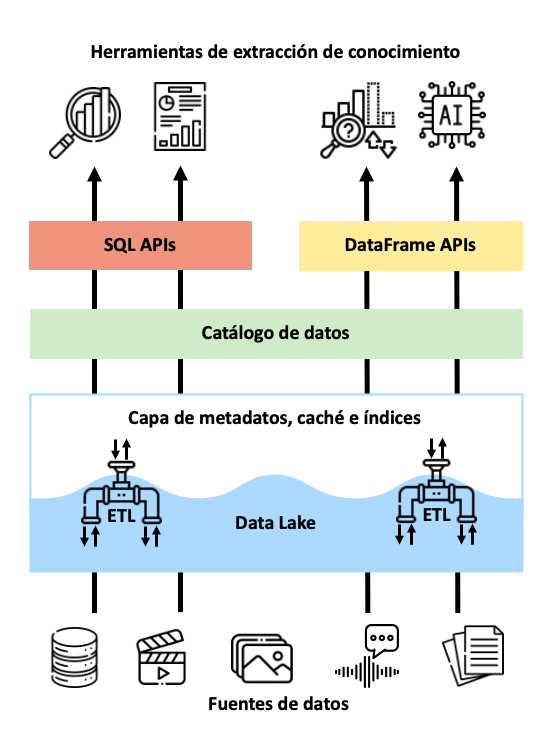
\includegraphics[width=0.5\textwidth]{Images/dlh-architecture.png}
    \caption{Arquitectura básica de un \textit{data lakehouse}}
    \label{fig:dlh-architecture}
\end{figure}




\begin{longtable}{|p{3cm}|p{4cm}|p{4cm}|p{4cm}|}
    \hline
    \textbf{Criterio}         & \textbf{Data warehouse}                                   & \textbf{Data lake}                                                       & \textbf{Data lakehouse}                                                  \\ \hline
    \endfirsthead
    \hline
    \textbf{Criterio}         & \textbf{Data warehouse}                                   & \textbf{Data lake}                                                       & \textbf{Data lakehouse}                                                  \\ \hline
    \endhead
    \hline
    \multicolumn{4}{|r|}{Continúa en la siguiente página...} \\ \hline
    \endfoot
    \hline
    \endlastfoot
    \textbf{Enfoque clave}    & Análisis de datos e inteligencia empresarial                & Exploración de datos, análisis de grandes datos y fuente única de verdad para diversos tipos de datos (e.g., registros, documentos, multimedia) & Combina análisis de datos estructurados con gestión transaccional            \\ \hline
    \textbf{Tipo de datos}    & Estructurados                                               & Estructurados, semi-estructurados y no estructurados                         & Estructurados, semi-estructurados y no estructurados                         \\ \hline
    \textbf{Costo de almacenamiento}            & Costoso y lento                                             & Económico, rápido y adaptable                                                & Económico, rápido y adaptable                                                \\ \hline
    \textbf{Estructura}       & No configurable                                             & Personalizable                                                               & Personalizable                                                               \\ \hline
    \textbf{Esquema}          & Definido antes de almacenar los datos (esquema en escritura) & Desarrollado después de almacenar los datos (esquema en lectura)             & Desarrollado después de almacenar los datos (esquema en lectura)             \\ \hline
    \textbf{Cumplimiento de esquema} & Estricto                                              & Flexible                                                                     & Flexible                                                                     \\ \hline
    \textbf{Usabilidad}       & Los usuarios pueden acceder y reportar datos fácilmente     & Complejo analizar grandes volúmenes de datos sin herramientas de clasificación y catalogación & Combina la estructura y simplicidad del almacén de datos con los casos de uso más amplios del lago de datos \\ \hline
    \textbf{Conformidad ACID} & Garantiza altos niveles de integridad, los datos se registran de manera compatible con ACID & No cumple con ACID, las actualizaciones y eliminaciones son procedimientos complejos & Compatible con ACID para garantizar consistencia en operaciones concurrentes de lectura/escritura \\ \hline
    \textbf{Calidad}          & Alta                                                        & Riesgo de baja calidad (pantanos de datos) si no se gestiona correctamente   & Alta                                                                         \\ \hline
    \textbf{Gobernanza de datos} & Funciones integradas para calidad e integridad de datos   & Requiere herramientas adicionales para una gobernanza efectiva              & Enfoque híbrido, aprovecha las características del almacén de datos para una mejor gobernanza \\ \hline
    \textbf{Escalabilidad}    & Escalado vertical                                           & Escalado horizontal                                                          & Escalado horizontal                                                          \\ \hline
    \end{longtable}



\subsubsection{Arquitecturas de integración de datos virtual}


\paragraph{Logical data warehouse\newline}


El \textit{logical data warehouse} (LDW)
es una arquitectura en la que se implementa una capa de virtualización de datos
encima de sistemas de integración de datos o fuentes primarias de datos. Esto
permite tanto el acceso a datos reconciliados como datos en tiempo real haciendo que
estas fuentes se presenten al usuario como una única fuente de datos. Esto permite 
consultar tanto las fuentes de datos convencionales (como bases de datos, almacenes de datos empresariales, lagos de datos, etc.) 
como otras fuentes de datos (como aplicaciones, archivos de big data, servicios web y la nube) para satisfacer cualquier caso de uso analítico.

Un LDW no almacena datos físicamente, sino que contiene metadatos que definen el contexto de los datos, lo que permite a los consumidores de datos encontrar y acceder a una pieza específica de datos sin necesidad de saber dónde está almacenada.
Esto permite no utilizar procesos ETL o ELT físicos, es decir no se copian o mueven los datos a un almacenamiento
centralizado. En este caso se utilizan los mapeos semánticos entre un esquema mediador global y los esquemas de las fuentes
de datos para reformular las consultas del usuario y distribuirlas a las distintas fuentes.

La arquitectura básica de un data warehouse lógico se compone de los siguientes componentes:

\begin{itemize}
    \item Capa de metadatos: Incluye el El esquema mediado se construye para la aplicación de integración de datos y contiene únicamente los aspectos del dominio que son relevantes para la aplicación. La clave para construir una aplicación de integración de datos son las descripciones de las fuentes, el vínculo que conecta el esquema mediado con los esquemas de las fuentes. Estas descripciones especifican las propiedades de las fuentes que el sistema necesita conocer para poder utilizar sus datos. El componente principal de las descripciones de las fuentes son los mapeos semánticos, que relacionan los esquemas de las fuentes de datos con el esquema mediado. Los mapeos semánticos especifican cómo los atributos de las fuentes corresponden a los atributos del esquema mediado (cuando existen tales correspondencias) y cómo se resuelven las diferentes agrupaciones de atributos en tablas.
    \item Reformulador de consultas: Por lo tanto, el primer paso que debe realizar el sistema es reformular la consulta en consultas que se refieran a los esquemas de las fuentes de datos. Para ello, el sistema utiliza las descripciones de las fuentes. El resultado de la reformulación es un conjunto de consultas que hacen referencia a los esquemas de las fuentes de datos y cuya combinación producirá la respuesta a la consulta original.
    \item Optimizador de consultas:  La optimización de consultas toma como entrada un plan de consulta lógico y produce un plan de consulta física, que especifica el orden exacto en que se acceden a las fuentes de datos, cuándo se combinan los resultados, qué algoritmos se utilizan para realizar operaciones sobre los datos (por ejemplo, uniones entre fuentes) y la cantidad de recursos asignados a cada operación.
    \item Motor de ejecución: el motor de ejecución es responsable de la ejecución real del plan de consulta física. El motor de ejecución envía las consultas a las fuentes individuales a través de los envoltorios (wrappers) y combina los resultados según lo especificado por el plan de consulta.
    \item Decoradores: su función es extraer los metadatos, enviar consultas a una fuente de datos, recibir las respuestas,
    
\end{itemize}

\begin{figure}[h!]
    \centering
    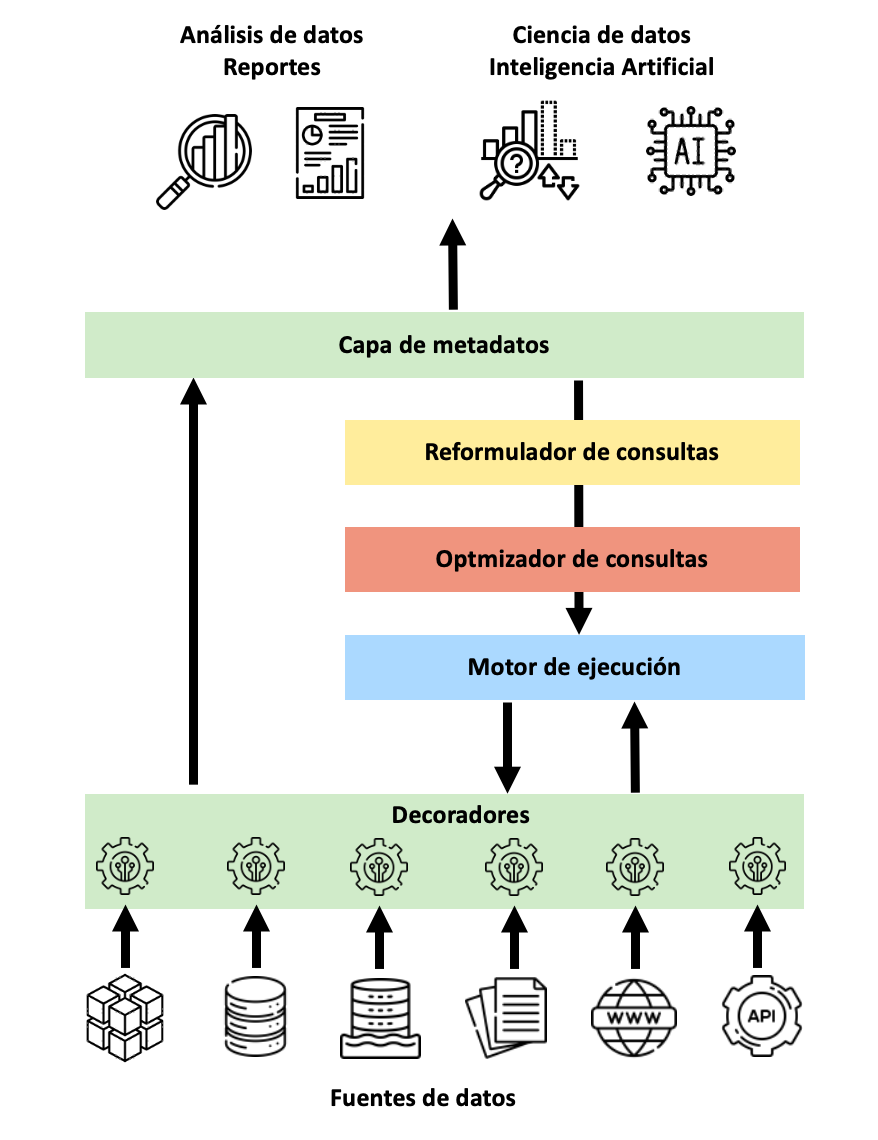
\includegraphics[width=0.5\textwidth]{Images/ldw-architecture.png}
    \caption{Arquitectura de un \textit{logical data warehouse}}
    \label{fig:ldw-architecture}
\end{figure}

\subsubsection{Integración física vs. integración virtual}

\begin{longtable}{|p{3cm}|p{4.5cm}|p{4.5cm}|}
    \hline
    \textbf{Aspecto} & \textbf{Integración de Datos Física} & \textbf{Integración de Datos Virtual} \\
    \hline
    Definición & Copia y consolida los datos desde múltiples fuentes en un único repositorio central (p. ej., un almacén de datos). & Proporciona acceso a los datos en múltiples fuentes sin moverlos físicamente, utilizando una capa lógica. \\
    \hline
    Almacenamiento & Los datos se almacenan físicamente en un repositorio común (almacén de datos o data lake). & Los datos permanecen en sus fuentes originales; no se duplican ni consolidan físicamente. \\
    \hline
    Rendimiento & Alto rendimiento para consultas complejas debido a la pre-optimización de datos. & El rendimiento depende de la capacidad de las fuentes y la eficiencia de las consultas distribuidas. \\
    \hline
    Tiempo de implementación & Requiere tiempo considerable para la extracción, transformación y carga (ETL/ELT) de los datos. & Implementación más rápida, ya que no es necesario mover ni transformar los datos previamente. \\
    \hline
    Actualización de datos & Los datos no están en tiempo real; las actualizaciones dependen de la frecuencia de los procesos ETL/ELT. & Los datos están siempre en tiempo real, ya que se accede directamente a las fuentes originales. \\
    \hline
    Escalabilidad & Requiere aumentar el almacenamiento y la capacidad de procesamiento a medida que crecen los datos. & Más escalable, ya que aprovecha el almacenamiento y procesamiento de las fuentes individuales. \\
    \hline
    Complejidad de mantenimiento & Complejo; requiere mantenimiento de ETL/ELT, además de la gestión del repositorio central. & Más simple, ya que no se duplican los datos, pero puede ser complicado manejar múltiples fuentes heterogéneas. \\
    \hline
    Consistencia de datos & Alta consistencia si los procesos ETL/ELT están bien diseñados. & Puede haber problemas de consistencia debido a diferencias entre las fuentes en tiempo real. \\
    \hline
    Casos de uso & Ideal para análisis históricos, minería de datos, y reportes empresariales en grandes organizaciones. & Adecuado para consultas en tiempo real y aplicaciones que necesitan acceso inmediato a datos actualizados. \\
    \hline
    Costo inicial & Alto, debido al almacenamiento físico y la implementación de procesos ETL/ELT. & Menor costo inicial, pero requiere inversión en herramientas de virtualización y gestión de consultas. \\
    \hline
    \end{longtable}




